% Options for packages loaded elsewhere
\PassOptionsToPackage{unicode}{hyperref}
\PassOptionsToPackage{hyphens}{url}
\documentclass[
  11pt,
]{article}
\usepackage{xcolor}
\usepackage[a4paper,margin=22mm]{geometry}
\usepackage{amsmath,amssymb}
\setcounter{secnumdepth}{-\maxdimen} % remove section numbering
\usepackage{iftex}
\ifPDFTeX
  \usepackage[T1]{fontenc}
  \usepackage[utf8]{inputenc}
  \usepackage{textcomp} % provide euro and other symbols
\else % if luatex or xetex
  \usepackage{unicode-math} % this also loads fontspec
  \defaultfontfeatures{Scale=MatchLowercase}
  \defaultfontfeatures[\rmfamily]{Ligatures=TeX,Scale=1}
\fi
\usepackage{lmodern}
\ifPDFTeX\else
  % xetex/luatex font selection
\fi
% Use upquote if available, for straight quotes in verbatim environments
\IfFileExists{upquote.sty}{\usepackage{upquote}}{}
\IfFileExists{microtype.sty}{% use microtype if available
  \usepackage[]{microtype}
  \UseMicrotypeSet[protrusion]{basicmath} % disable protrusion for tt fonts
}{}
\makeatletter
\@ifundefined{KOMAClassName}{% if non-KOMA class
  \IfFileExists{parskip.sty}{%
    \usepackage{parskip}
  }{% else
    \setlength{\parindent}{0pt}
    \setlength{\parskip}{6pt plus 2pt minus 1pt}}
}{% if KOMA class
  \KOMAoptions{parskip=half}}
\makeatother
\usepackage{longtable,booktabs,array}
\newcounter{none} % for unnumbered tables
\usepackage{calc} % for calculating minipage widths
% Correct order of tables after \paragraph or \subparagraph
\usepackage{etoolbox}
\makeatletter
\patchcmd\longtable{\par}{\if@noskipsec\mbox{}\fi\par}{}{}
\makeatother
% Allow footnotes in longtable head/foot
\IfFileExists{footnotehyper.sty}{\usepackage{footnotehyper}}{\usepackage{footnote}}
\makesavenoteenv{longtable}
\setlength{\emergencystretch}{3em} % prevent overfull lines
\providecommand{\tightlist}{%
  \setlength{\itemsep}{0pt}\setlength{\parskip}{0pt}}
\usepackage{float,caption,tikz,pgfplots}
\usepgfplotslibrary{groupplots}
\pgfplotsset{compat=1.18}
\setlength{\parskip}{.45em}
\setlength{\parindent}{0pt}
\setlength{\emergencystretch}{3em}
\pagestyle{plain}
\usepackage{bookmark}
\IfFileExists{xurl.sty}{\usepackage{xurl}}{} % add URL line breaks if available
\urlstyle{same}
\hypersetup{
  pdftitle={Nucleus-center localization: experimental results and object-level analysis --- Stage report 8},
  pdfauthor={bdd26 research},
  hidelinks,
  pdfcreator={LaTeX via pandoc}}

\title{Nucleus-center localization: experimental results and
object-level analysis --- Stage report 8}
\author{bdd26 research}
\date{17 November 2026}

\begin{document}
\maketitle

{
\setcounter{tocdepth}{2}
\tableofcontents
\newpage
}
\subsection{Research question and
findings}\label{research-question-and-findings}

Stage report 7 covered experiments through P26. This report follows P27
through P31, describing each question, paired control, training and
development results, and the annotated nuclei in fixed images. P27--P30
compare which layers of a pretrained image encoder are updated; P31
retains last-twelve encoder updates and adds group normalization to the
center detector.

Each experiment uses 2,134 training images and a separate set of 522
development images from PanNuke fold 1. The development images contain
12,250 annotated nuclei, including 145 apoptotic or necrotic nuclei
whose outlines do not touch an image boundary; these occur in 11 images,
and 32 have area below 67 square pixels. Predicted and annotated centers
are assigned one-to-one within three native pixels. Recall is the
fraction of annotated nuclei matched, precision is the fraction of
predictions matched, and unmatched predictions are additional output
points. Each paired control and intervention was trained independently
for 130 epochs with seeds 19 and 1; the last checkpoint was evaluated.

Relative to its own control, P27 added 6/15 interior Dead matches, P28
changed them by +2/−1, P29 added 16/13, P30 added 7/15 and P31 added
8/2. P30 added 648/516 all-nucleus matches while reducing unmatched
predictions by 215/254; P31 changed all matches by −140/+6. The chart
compares the five rounds; the image analyses identify the individual
gains and losses behind the totals.

\begin{figure}[H]\centering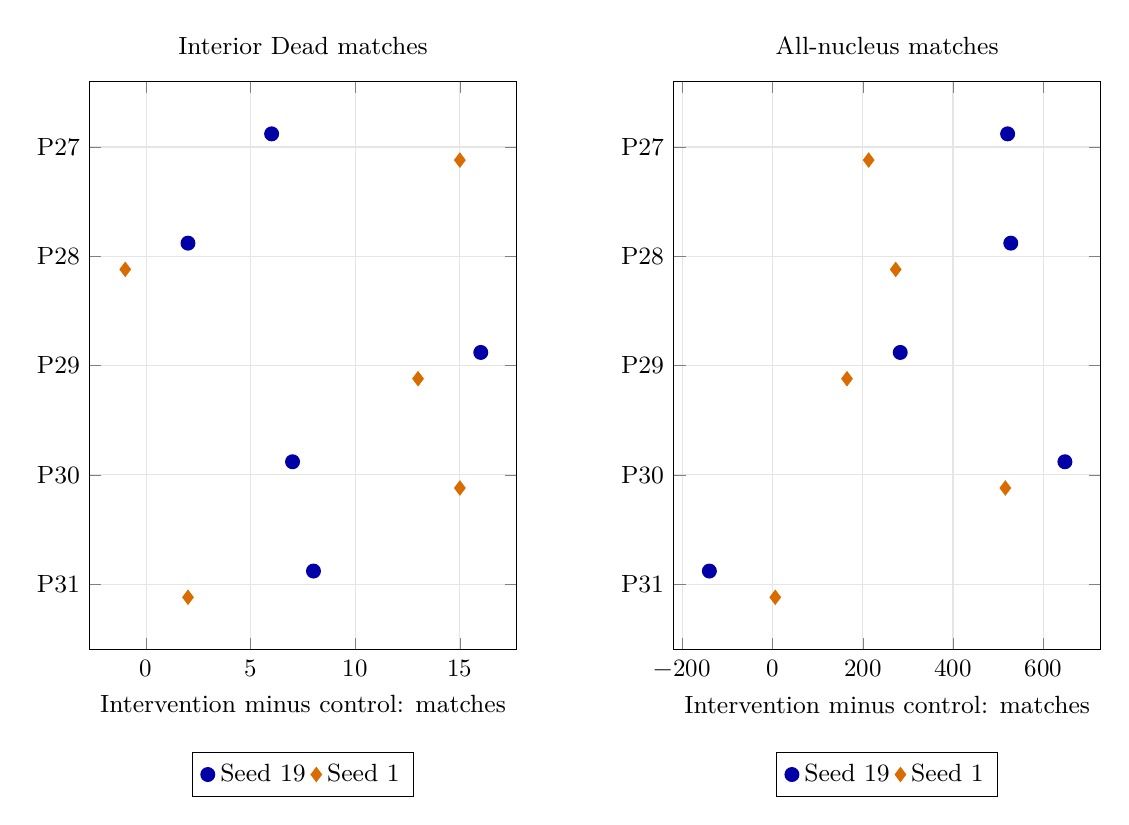
\begin{tikzpicture}
\begin{groupplot}[group style={group size=2 by 1,horizontal sep=2.0cm},width=7cm,height=8.8cm,ytick={0,1,2,3,4},yticklabels={P27,P28,P29,P30,P31},ymin=-.6,ymax=4.6,y dir=reverse,grid=major,grid style={gray!20},tick label style={font=\small},label style={font=\small},title style={font=\small},legend style={font=\small,at={(.5,-.18)},anchor=north,legend columns=2}]
\nextgroupplot[title={Interior Dead matches},xlabel={Intervention minus control: matches}]
\addplot[only marks,mark=*,mark size=2.5pt,color=blue!65!black] coordinates {(6,-0.12) (2,0.88) (16,1.88) (7,2.88) (8,3.88)};
\addlegendentry{Seed 19}
\addplot[only marks,mark=diamond*,mark size=2.5pt,color=orange!85!black] coordinates {(15,0.12) (-1,1.12) (13,2.12) (15,3.12) (2,4.12)};
\addlegendentry{Seed 1}
\nextgroupplot[title={All-nucleus matches},xlabel={Intervention minus control: matches}]
\addplot[only marks,mark=*,mark size=2.5pt,color=blue!65!black] coordinates {(521,-0.12) (528,0.88) (283,1.88) (648,2.88) (-140,3.88)};
\addlegendentry{Seed 19}
\addplot[only marks,mark=diamond*,mark size=2.5pt,color=orange!85!black] coordinates {(213,0.12) (273,1.12) (165,2.12) (516,3.12) (6,4.12)};
\addlegendentry{Seed 1}
\end{groupplot}
\end{tikzpicture}
\caption{Intervention minus same-round control for P27–P31. Left: matched interior Dead nuclei. Right: matched nuclei of all types. Circles and diamonds indicate seeds 19 and 1.}\end{figure}

\subsection{P27: updating the first twelve
blocks}\label{p27-updating-the-first-twelve-blocks}

The control updates the last twelve encoder blocks; the intervention
updates the first twelve. Both have the same number of trainable encoder
parameters and share the remaining data, rates and detection protocol.

{\def\LTcaptype{none} % do not increment counter
\begin{longtable}[]{@{}
  >{\raggedright\arraybackslash}p{(\linewidth - 10\tabcolsep) * \real{0.1304}}
  >{\raggedleft\arraybackslash}p{(\linewidth - 10\tabcolsep) * \real{0.1739}}
  >{\raggedleft\arraybackslash}p{(\linewidth - 10\tabcolsep) * \real{0.1739}}
  >{\raggedleft\arraybackslash}p{(\linewidth - 10\tabcolsep) * \real{0.1739}}
  >{\raggedleft\arraybackslash}p{(\linewidth - 10\tabcolsep) * \real{0.1739}}
  >{\raggedleft\arraybackslash}p{(\linewidth - 10\tabcolsep) * \real{0.1739}}@{}}
\toprule\noalign{}
\begin{minipage}[b]{\linewidth}\raggedright
Seed and allocation
\end{minipage} & \begin{minipage}[b]{\linewidth}\raggedleft
Interior Dead
\end{minipage} & \begin{minipage}[b]{\linewidth}\raggedleft
Small Dead
\end{minipage} & \begin{minipage}[b]{\linewidth}\raggedleft
All matched / annotated
\end{minipage} & \begin{minipage}[b]{\linewidth}\raggedleft
Precision
\end{minipage} & \begin{minipage}[b]{\linewidth}\raggedleft
Unmatched
\end{minipage} \\
\midrule\noalign{}
\endhead
\bottomrule\noalign{}
\endlastfoot
19, last 12 & 72/145 & 10/32 & 7,264/12,250 & 69.41\% & 3,202 \\
19, first 12 & 78/145 & 9/32 & 7,785/12,250 & 74.25\% & 2,700 \\
1, last 12 & 65/145 & 6/32 & 7,395/12,250 & 69.49\% & 3,247 \\
1, first 12 & 80/145 & 10/32 & 7,608/12,250 & 74.89\% & 2,551 \\
\end{longtable}
}

Seed 19 produced only 19 more points while matching 521 more nuclei.
Seed 1 produced 483 fewer points while matching 213 more nuclei.
Training-set recall fell from 97.72\%/97.89\% to 88.80\%/87.82\%, and
final focal loss rose from 0.0563/0.0574 to 0.2643/0.2507. The
first-block recipe fit fewer training centers and matched more
development centers. Its gradients traverse the frozen later blocks, and
measured pure training time increased by 21\%/23\%. Allocated GPU memory
peaked at 4.84 GiB in the first-block runs and 4.05 GiB in controls.

Interior Dead recall gains were 4.14 and 10.34 percentage points. The
paired, tissue-stratified image bootstrap gave 95\% intervals of −0.57
to +15.38 and +1.85 to +15.49 points. Removing each Dead-positive image
in turn gave ranges of +2.31 to +10.42 and +8.46 to +14.17 points. Final
Dead recall was 53.79\%/55.17\% and precision was 74.25\%/74.89\%. The
original rule requires at least 60\% Dead recall and 75\% precision
among its criteria. Both seeds failed the complete rule, closing the
fixed first-12 recipe. The same development split has been reused across
rounds.

\subsubsection{Image and object changes}\label{image-and-object-changes}

Lung gained three matches in each seed. Cervix image 1756 gained three
and four, and esophagus image 2076 gained two in each seed. Colon image
1482 has 49 interior Dead annotations and moved from 17 to 13 matches in
seed 19 and 10 to 16 in seed 1. The eight fixed images contain 53
interior Dead objects. In seed 19, the first-block recipe retained 26,
gained 11, lost seven and missed nine in both arms. The corresponding
seed-1 counts were 26, six, seven and 14. The fixed subset therefore
gained four and lost one net, while the complete evaluation set gained
six and 15.

\noindent

\begin{minipage}{\linewidth}\centering
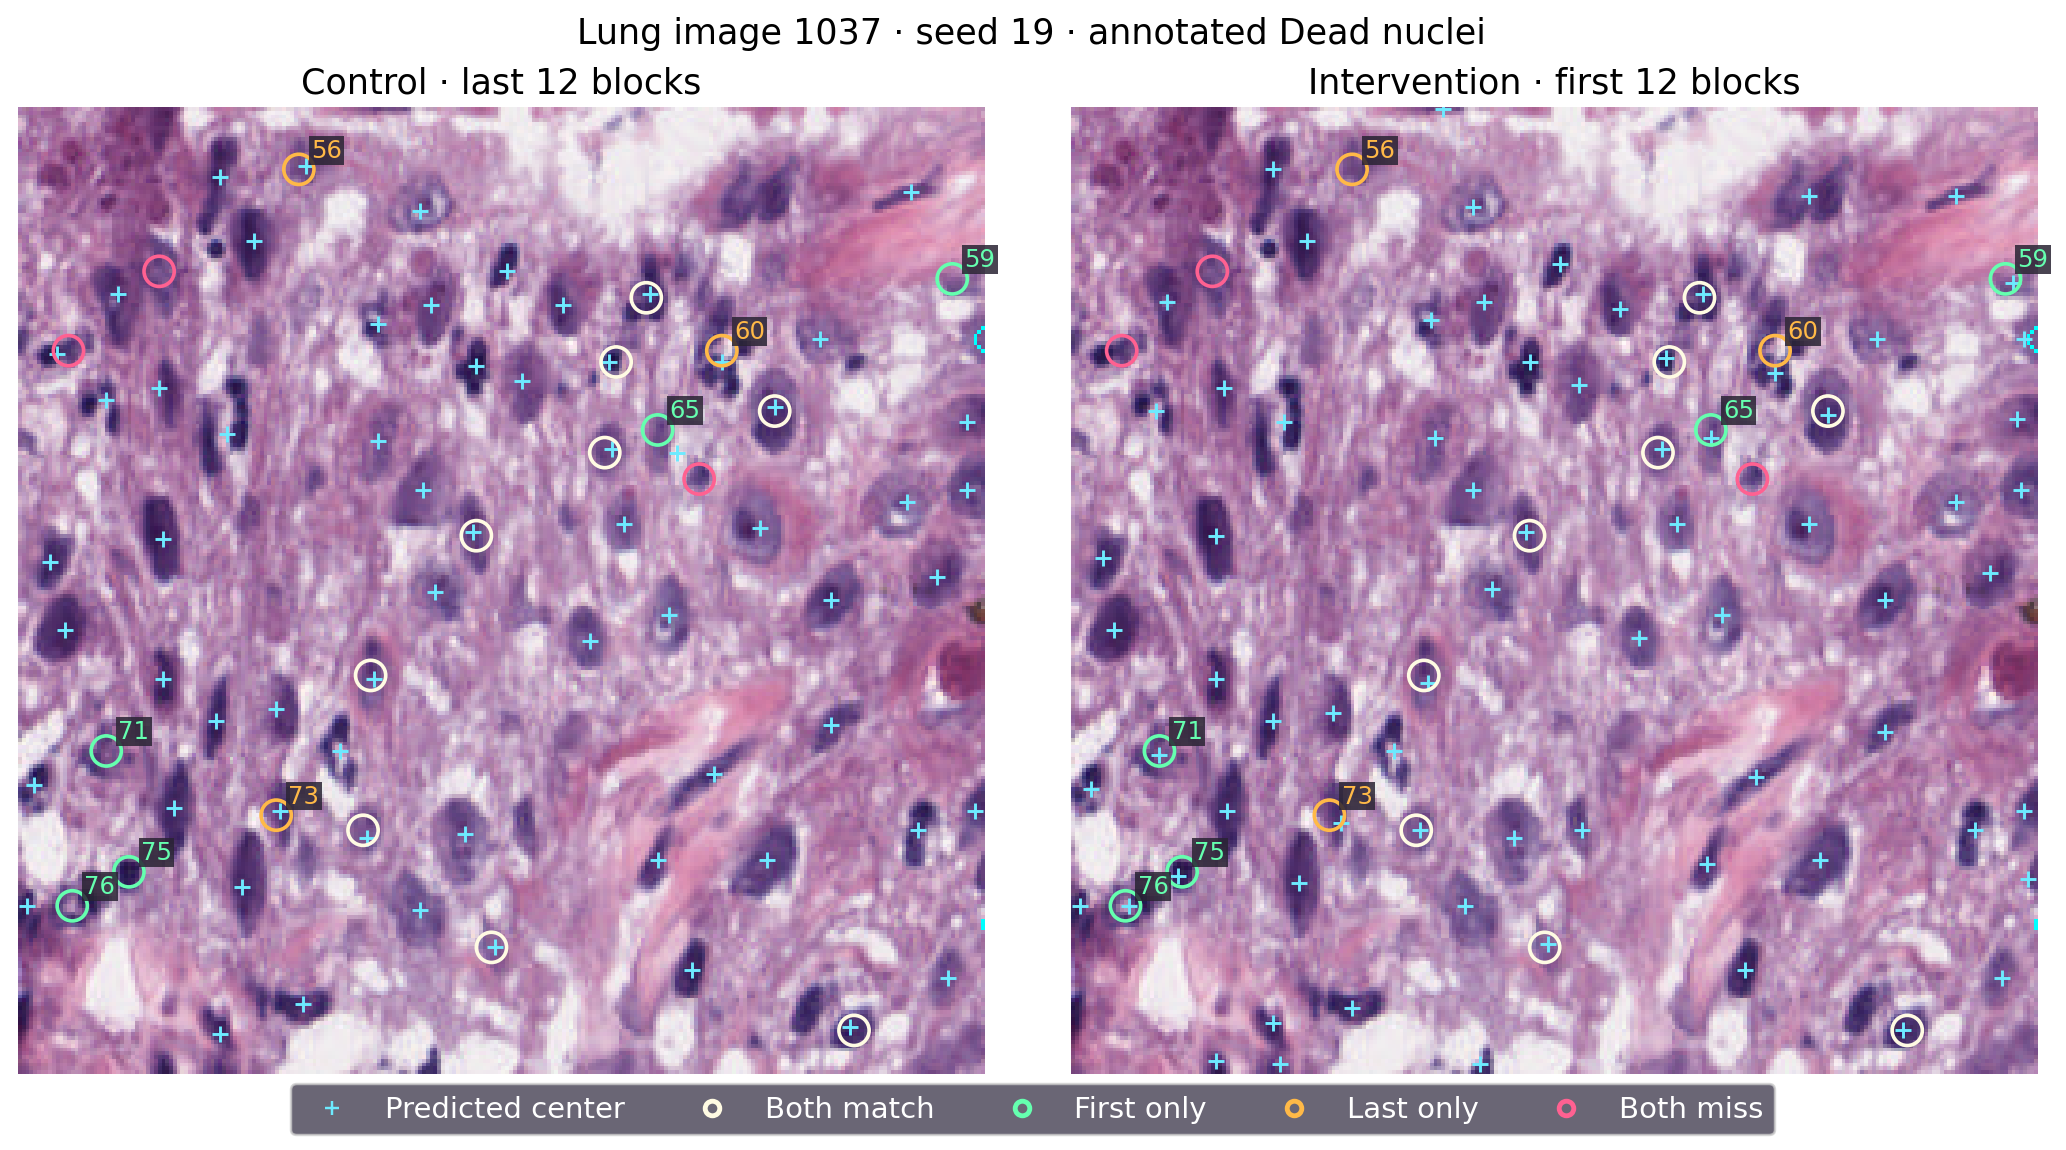
\includegraphics[width=\linewidth,height=.40\textheight,keepaspectratio]{assets/p27_image_1037_seed_19.png}
\captionof{figure}{Lung image 1037 in seed 19. Seed 19; last-twelve control left, first twelve intervention right. Cyan crosses mark predictions; white, green, orange and pink circles mark matched by both, intervention only, control only and missed by both}
\raggedright

Cyan crosses mark all predicted centers. Rings mark annotated interior Dead objects. Each ring has the same paired-outcome color in both panels. Lung image 1037 in seed 19 went from 12/20 to 14/20, with five newly matched objects and three lost. Object 65, at row 85 and column 169 beside a dark-stained region, gained a match as the nearest decoded point moved from 7.81 to 2.00 pixels away. Lower-left object 71 (170, 23) went from 21.02 to 1.00 pixel. Upper-left object 56 (16, 74) lost its match as the nearest point moved from 2.24 to 21.00 pixels away. For object 73 (187, 68), the distance changed from 1.41 to 3.61 pixels, crossing the match radius.

\end{minipage}

\noindent

\begin{minipage}{\linewidth}\centering
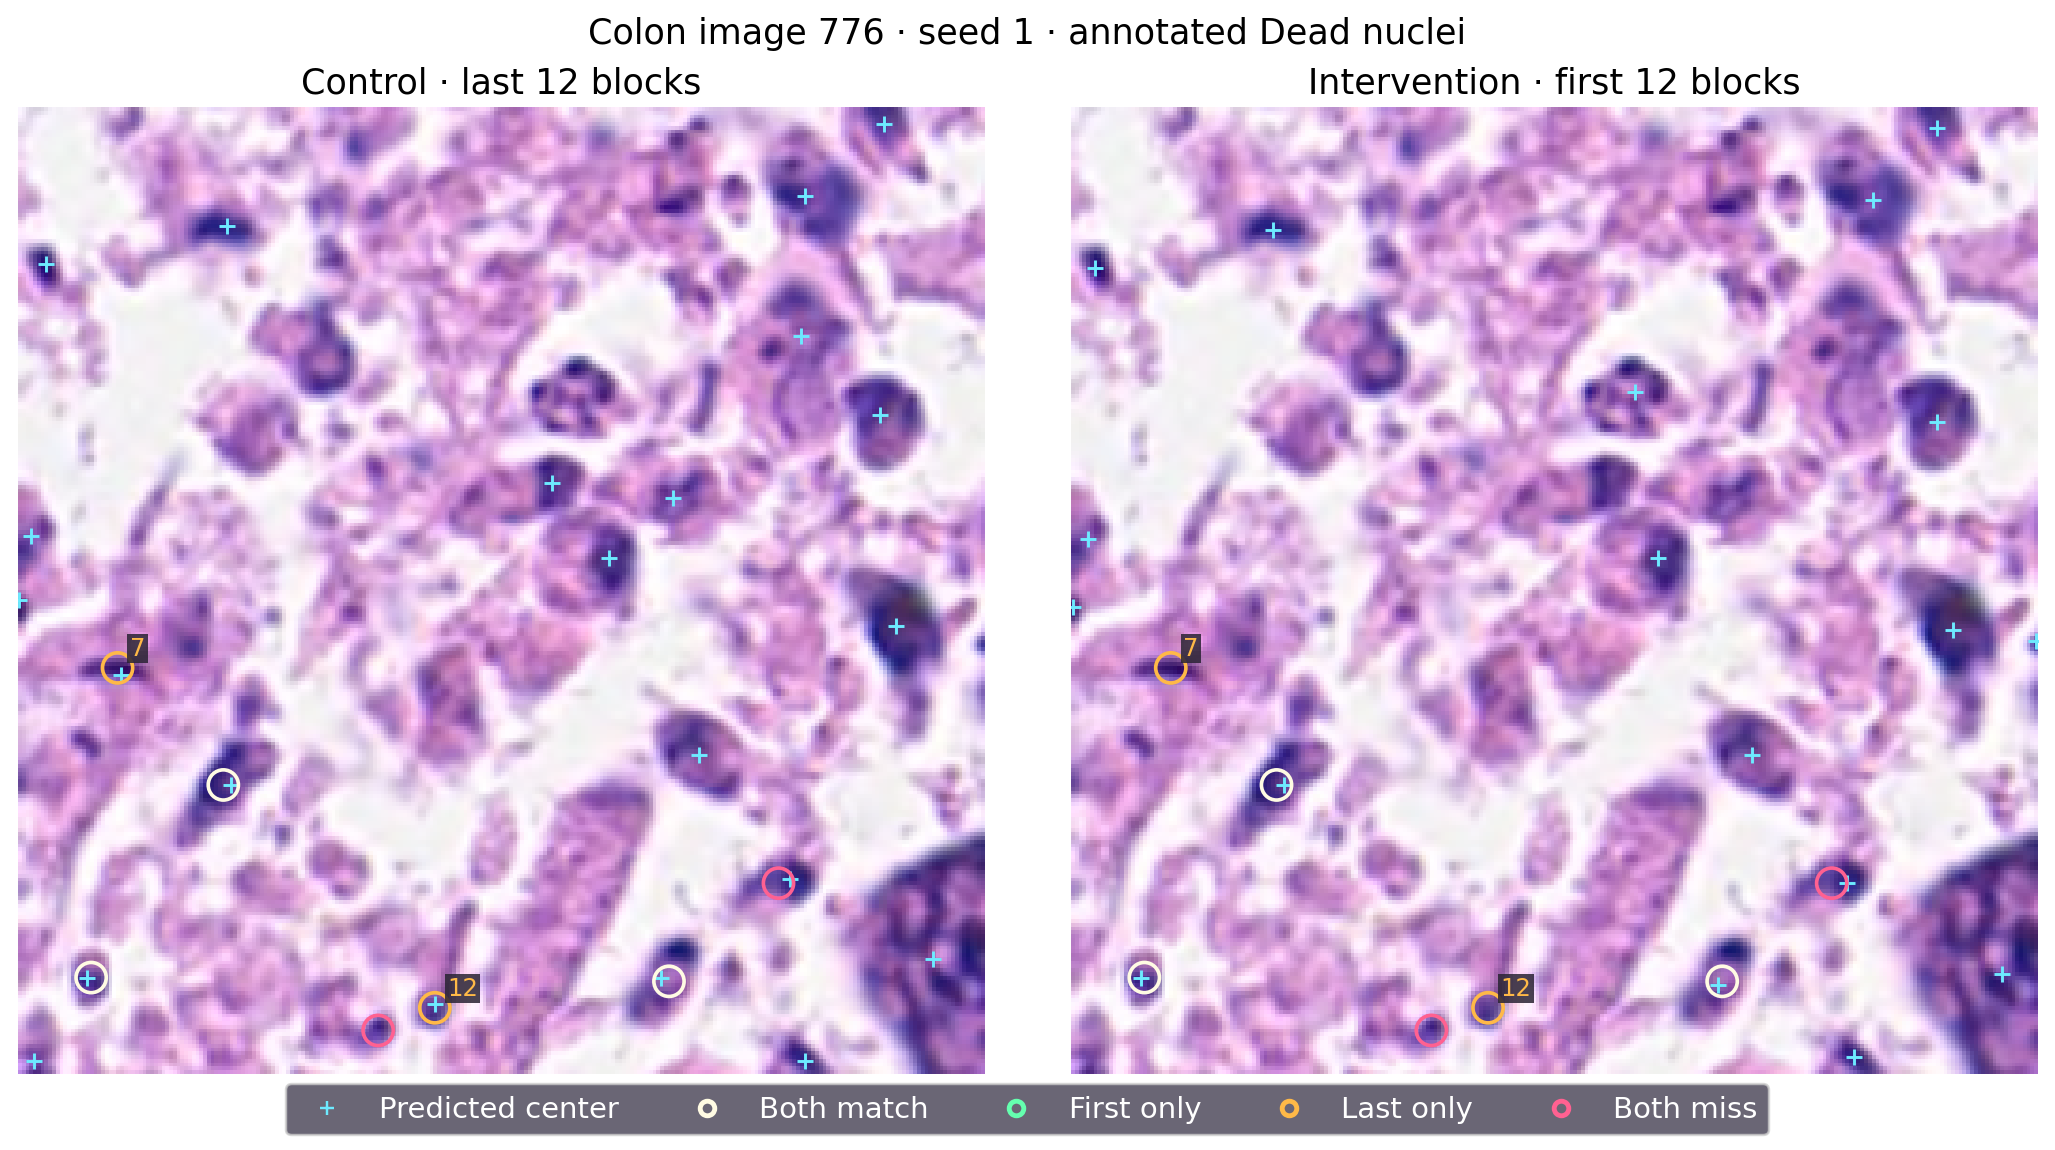
\includegraphics[width=\linewidth,height=.40\textheight,keepaspectratio]{assets/p27_image_776_seed_1.png}
\captionof{figure}{Colon image 776 in seed 1. Seed 1; last-twelve control left, first twelve intervention right. Cyan crosses mark predictions; white, green, orange and pink circles mark matched by both, intervention only, control only and missed by both}
\raggedright

Colon image 776 went from 5/7 to 3/7 in seed 1. Nearest-point distances for objects 7 (148, 26) and 12 (238, 110) increased from 2.24 to 30.53 and from 1.00 to 61.29 pixels. These locations lack nearby decoded outputs in the first-block arm. Object 8 (179, 54) matched (179, 56) in both arms. Nearby crosses at object 9 (205, 201) are 3.16 and 4.00 pixels away and fall outside the matching radius. Decoded distances distinguish near-radius shifts from the absence of nearby outputs. Separating weak scores, peak displacements and peak filtering requires complete score maps.

\end{minipage}

\subsection{P28: updating alternating
blocks}\label{p28-updating-alternating-blocks}

The control updates the last twelve encoder blocks. The intervention
updates zero-based blocks 1, 3, 5 through 23, keeping the same number of
trainable encoder parameters.

{\def\LTcaptype{none} % do not increment counter
\begin{longtable}[]{@{}
  >{\raggedright\arraybackslash}p{(\linewidth - 10\tabcolsep) * \real{0.1304}}
  >{\raggedleft\arraybackslash}p{(\linewidth - 10\tabcolsep) * \real{0.1739}}
  >{\raggedleft\arraybackslash}p{(\linewidth - 10\tabcolsep) * \real{0.1739}}
  >{\raggedleft\arraybackslash}p{(\linewidth - 10\tabcolsep) * \real{0.1739}}
  >{\raggedleft\arraybackslash}p{(\linewidth - 10\tabcolsep) * \real{0.1739}}
  >{\raggedleft\arraybackslash}p{(\linewidth - 10\tabcolsep) * \real{0.1739}}@{}}
\toprule\noalign{}
\begin{minipage}[b]{\linewidth}\raggedright
Seed and allocation
\end{minipage} & \begin{minipage}[b]{\linewidth}\raggedleft
Interior Dead
\end{minipage} & \begin{minipage}[b]{\linewidth}\raggedleft
Small Dead
\end{minipage} & \begin{minipage}[b]{\linewidth}\raggedleft
All matched
\end{minipage} & \begin{minipage}[b]{\linewidth}\raggedleft
Precision
\end{minipage} & \begin{minipage}[b]{\linewidth}\raggedleft
Unmatched
\end{minipage} \\
\midrule\noalign{}
\endhead
\bottomrule\noalign{}
\endlastfoot
19, last 12 & 68/145 & 7/32 & 7177/12,250 & 69.23\% & 3190 \\
19, odd-index 12 & 70/145 & 9/32 & 7705/12,250 & 71.24\% & 3110 \\
1, last 12 & 72/145 & 10/32 & 7361/12,250 & 69.07\% & 3296 \\
1, odd-index 12 & 71/145 & 9/32 & 7634/12,250 & 72.44\% & 2905 \\
\end{longtable}
}

Total recall rose 4.31/2.23 percentage points, and precision rose
2.01/3.36 points. Seed 19 emitted 448 more predictions, matching 528
more nuclei; seed 1 emitted 118 fewer predictions while matching 273
more. The first case primarily improves the usefulness of emitted
points; the second improves both their usefulness and count. Small Dead
matches changed 7 → 9 and 10 → 9.

Training-set recall changed 97.91\% → 96.32\% and 97.89\% → 96.31\%.
Final focal loss changed 0.05339 → 0.08767 and 0.05474 → 0.08310. Pure
training took 4.009/4.020 hours for controls and 4.781/4.757 hours for
alternate blocks, an increase of 19.27\%/18.33\%. Peak allocated GPU
memory was 4.05 versus 4.78 GiB. Scheduler elapsed time totaled 18:19:46
(18.3294 GPUh) across the four jobs, including startup, checkpointing
and preservation. Pure training time and scheduler accounting answer
different cost questions.

The original image bootstrap was independently recomputed against the
saved admission function. Dead recall gains were 1.38/−0.69 percentage
points, with 95\% intervals {[}−6.29,+13.27{]}/{[}−2.54,+2.34{]} points.
Final Dead recall 48.28\%/48.97\%, gain and lower-bound requirements,
and final precision 71.24\%/72.44\% were below the fixed criteria. Both
seeds failed the full conjunction; the exact odd-index recipe closes.

\subsubsection{Tissue and object
changes}\label{tissue-and-object-changes}

Lung's aggregate change was+6/0; colon changed−4/−1. Seed 19 lung image
1038 added five matches, while colon image 1482 lost four. The colon
image contains 49 of 145 interior Dead objects (33.79\% of support).
Removing this image descriptively changes seed 19's gain to 6/96=6.25\%;
removing lung 1038 changes it to −3/130=−2.31\%. Seed 1 leave-one-image
changes range from−1.54\% to 0.00\%. These sensitivity calculations
quantify concentration while retaining all 11 images in the actual
decision.

The pre-fixed eight examples contain 53 interior Dead objects. Seed 19
retained 26, gained 7, lost 6 and missed 14 in both arms. Seed 1
retained 28, gained 5, lost 5 and missed 15. Their net changes are+1/0,
compared with+2/−1 in the complete 522-image evaluation. Fixed examples
explain individual events; the complete image set determines the
aggregate result.

\noindent

\begin{minipage}{\linewidth}\centering
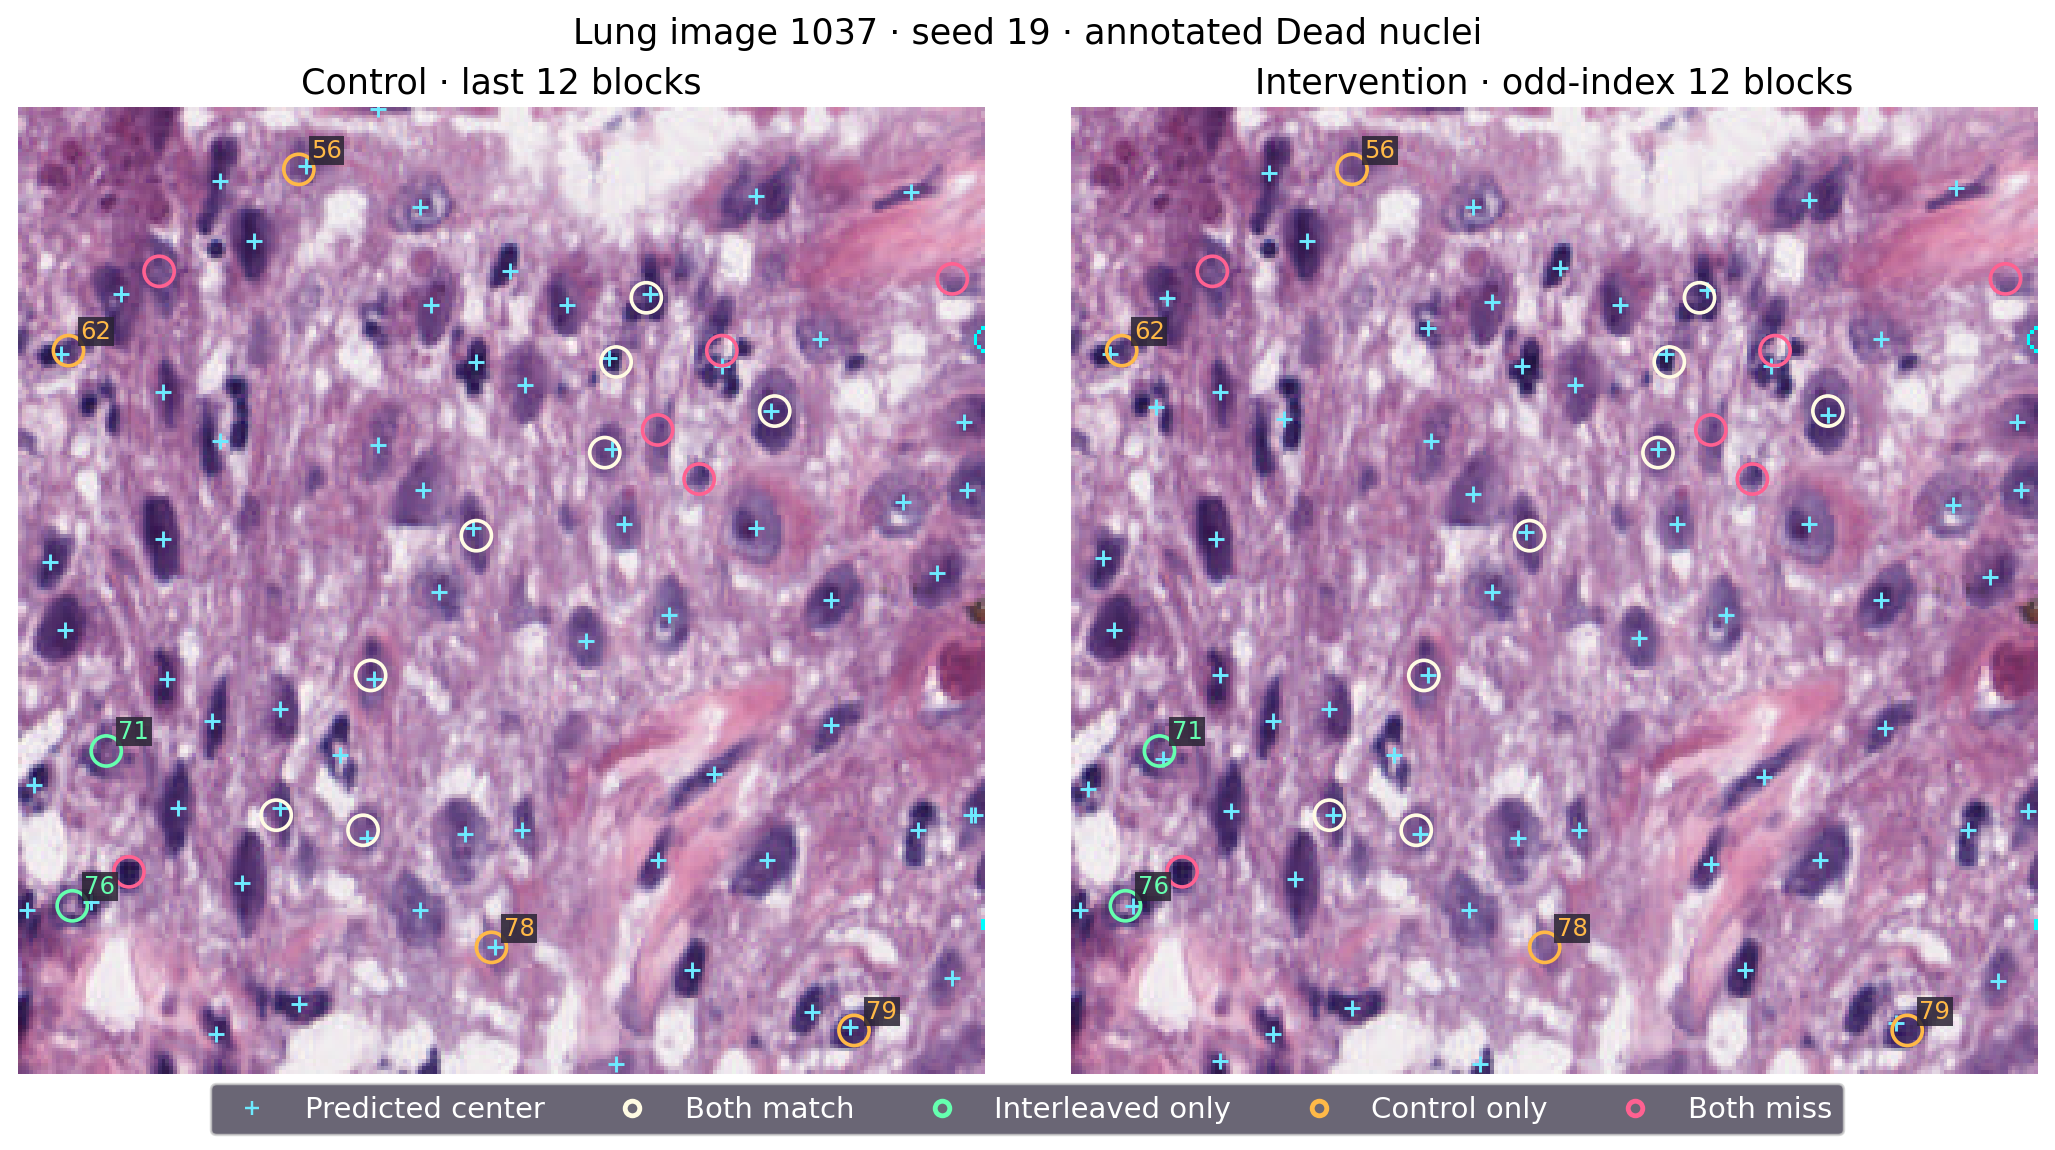
\includegraphics[width=\linewidth,height=.40\textheight,keepaspectratio]{assets/p28_image_1037_seed_19.png}
\captionof{figure}{Lung image 1037, seed 19; identical object colors in both panels. Seed 19; last-twelve control left, alternating twelve intervention right. Cyan crosses mark predictions; white, green, orange and pink circles mark matched by both, intervention only, control only and missed by both}
\raggedright

Cyan crosses are all decoded predictions. White rings identify Dead objects matched by both models, green rings those matched only by alternating updates, orange rings those matched only by control, and pink rings misses in both. Labels index the preserved GT list in fixed\_objects.csv; coordinates use row,column.

\end{minipage}

In lung image 1037 seed 19, matches changed 12 → 10: two objects gained
a match and four lost one. Object 71 at(170,23), in the lower-left
tissue, changed nearest-point distance 21.02 → 2.24 pixels. Object 76
at(211,14) changed 5.10 → 2.00. Conversely, upper-left object 56
at(16,74) changed 2.24 → 22.02, and lower object 78 at(222,125) changed
1.00 → 22.36; the intervention has no nearby decoded output at those
annotations. Object 62 at(64,13) changed 2.24 → 3.16 and object 79
at(244,221) changed 1.41 → 3.61. These latter losses arise at the
three-pixel matching boundary: visually nearby points can remain outside
the assigned radius.

\noindent

\begin{minipage}{\linewidth}\centering
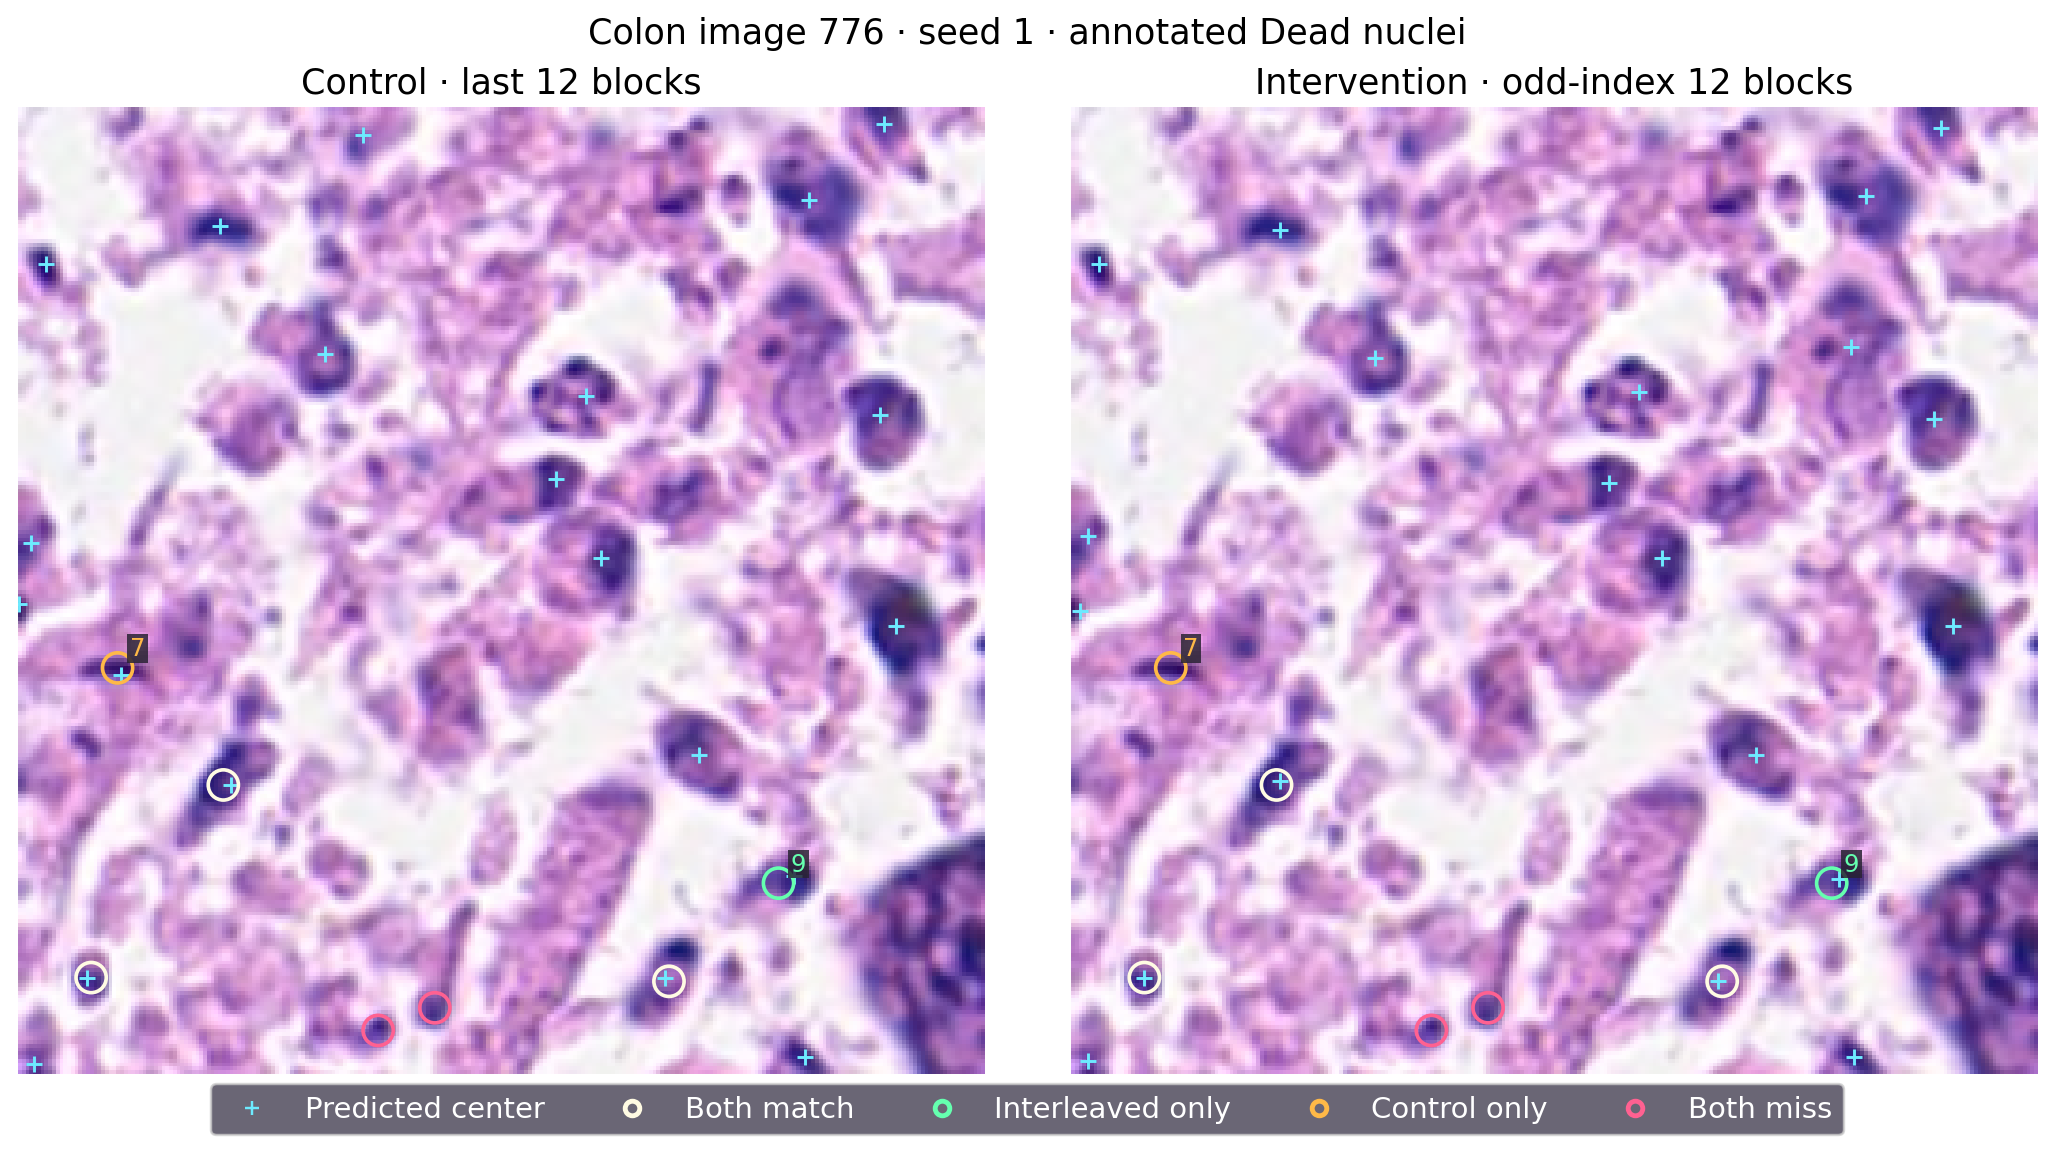
\includegraphics[width=\linewidth,height=.40\textheight,keepaspectratio]{assets/p28_image_776_seed_1.png}
\captionof{figure}{Colon image 776, seed 1: exchanged objects despite an unchanged total. Seed 1; last-twelve control left, alternating twelve intervention right. Cyan crosses mark predictions; white, green, orange and pink circles mark matched by both, intervention only, control only and missed by both}
\raggedright

Colon image 776 stayed at 4/7 Dead matches in both seeds, with one gained and one lost object. Object 7 at(148,26) lost its nearby prediction in both seeds: nearest distance became 28.30 pixels, from 2.83/2.24. Object 9 at(205,201) gained a match at(204,203), distance 2.24, from control distances 3.16/4.47. A constant image count therefore conceals substitution of which nuclei are found. The loss at object 7 concerns absence of a nearby decoded point; the gain at object 9 involves a point entering the match neighborhood.

\end{minipage}

The dark nuclear outlines, stain gradients and crowded tissue in the
panels provide spatial context. Decoded coordinates establish point
disappearance and displacement. Future probability-map and feature
measurements can distinguish center scores from peak selection. The
original four-panel PNGs also preserve response previews.

\subsection{P29: updating the first six and last six
blocks}\label{p29-updating-the-first-six-and-last-six-blocks}

The control updates the last twelve encoder blocks; the intervention
updates the first six and last six, retaining the same trainable
parameter count.

{\def\LTcaptype{none} % do not increment counter
\begin{longtable}[]{@{}
  >{\raggedright\arraybackslash}p{(\linewidth - 12\tabcolsep) * \real{0.1111}}
  >{\raggedleft\arraybackslash}p{(\linewidth - 12\tabcolsep) * \real{0.1481}}
  >{\raggedleft\arraybackslash}p{(\linewidth - 12\tabcolsep) * \real{0.1481}}
  >{\raggedleft\arraybackslash}p{(\linewidth - 12\tabcolsep) * \real{0.1481}}
  >{\raggedleft\arraybackslash}p{(\linewidth - 12\tabcolsep) * \real{0.1481}}
  >{\raggedleft\arraybackslash}p{(\linewidth - 12\tabcolsep) * \real{0.1481}}
  >{\raggedleft\arraybackslash}p{(\linewidth - 12\tabcolsep) * \real{0.1481}}@{}}
\toprule\noalign{}
\begin{minipage}[b]{\linewidth}\raggedright
Group
\end{minipage} & \begin{minipage}[b]{\linewidth}\raggedleft
Interior Dead
\end{minipage} & \begin{minipage}[b]{\linewidth}\raggedleft
Small Dead
\end{minipage} & \begin{minipage}[b]{\linewidth}\raggedleft
All matched
\end{minipage} & \begin{minipage}[b]{\linewidth}\raggedleft
Recall
\end{minipage} & \begin{minipage}[b]{\linewidth}\raggedleft
Precision
\end{minipage} & \begin{minipage}[b]{\linewidth}\raggedleft
Unmatched
\end{minipage} \\
\midrule\noalign{}
\endhead
\bottomrule\noalign{}
\endlastfoot
Last 12 blocks & 65/145 & 7/32 & 7,257/12,250 & 59.24\% & 69.73\% &
3,150 \\
First 6 + last 6 & 81/145 & 11/32 & 7,540/12,250 & 61.55\% & 70.96\% &
3,085 \\
\end{longtable}
}

The intervention emitted 218 more points while finding 283 more nuclei.
This combination reflects more useful predictions rather than a simple
increase in output count. Interior Dead recall rose 11.0345 percentage
points, with the unchanged 1,000-draw tissue-stratified bootstrap
interval {[}+3.0457,+27.9570{]} points. Overall recall rose 2.3102
points and precision 1.2328 points. The original seed-level conjunction
fails the absolute Dead recall (.60) and precision (.75) clauses; all
other seed-19 clauses pass. The seed-1 comparison independently improves
Dead recall by 8.9655 percentage points and also fails the same two
absolute clauses.

Training recall changed 97.51\% → 95.47\% and training Dead coverage
630/656 → 607/656. Pure training took 4.0130 versus 4.8652 hours, a
21.24\% increase. Peak allocated GPU memory was 4.05 versus 4.84 GiB.
Completed seed-19 scheduler elapsed time was 4:13:24 plus 5:00:21,
including startup, evaluation and preservation. These measurements price
the twelve-block intervention without substituting training fit for
development performance.

\subsubsection{Tissue distribution and
sensitivity}\label{tissue-distribution-and-sensitivity}

Six images gained matches, one lost matches and four were unchanged.
Lung changed +4, colon +3, cervix +2, esophagus +5 and stomach +2;
breast and uterus were unchanged. Lung image 1038 and esophagus image
2076 each gained five, together accounting for 10/16 net gains. Lung
image 1025 lost two despite aggregate lung improvement. Colon image 1482
contains 49/145 target objects and stays at 13 matches in both arms,
leaving 36 unmatched target objects in that image.

Removing one Dead-positive image at a time, solely as a sensitivity
calculation, leaves gains between 8.03\% and 16.67\%. Every such gain
remains positive. The observed seed-19 sign consequently survives
omission of any one contributing image; the full original decision still
includes all eleven images. A tissue with one positive image offers
limited evidence for between-image consistency within that tissue.

\subsubsection{Fixed images: which annotated nuclei
changed}\label{fixed-images-which-annotated-nuclei-changed}

The pre-fixed eight evaluation examples contain 53 interior Dead nuclei.
Seed 19 retained 30, gained 6, lost 4 and missed 13 in both arms. Their
net change is +2, versus +16 across all 522 evaluation images. Object
indices and row,column coordinates are retained in fixed\_objects.csv.
Cyan crosses show all predictions; shared white, green, orange and pink
rings respectively identify retained, gained, lost and jointly missed
target objects.

\noindent

\begin{minipage}{\linewidth}\centering
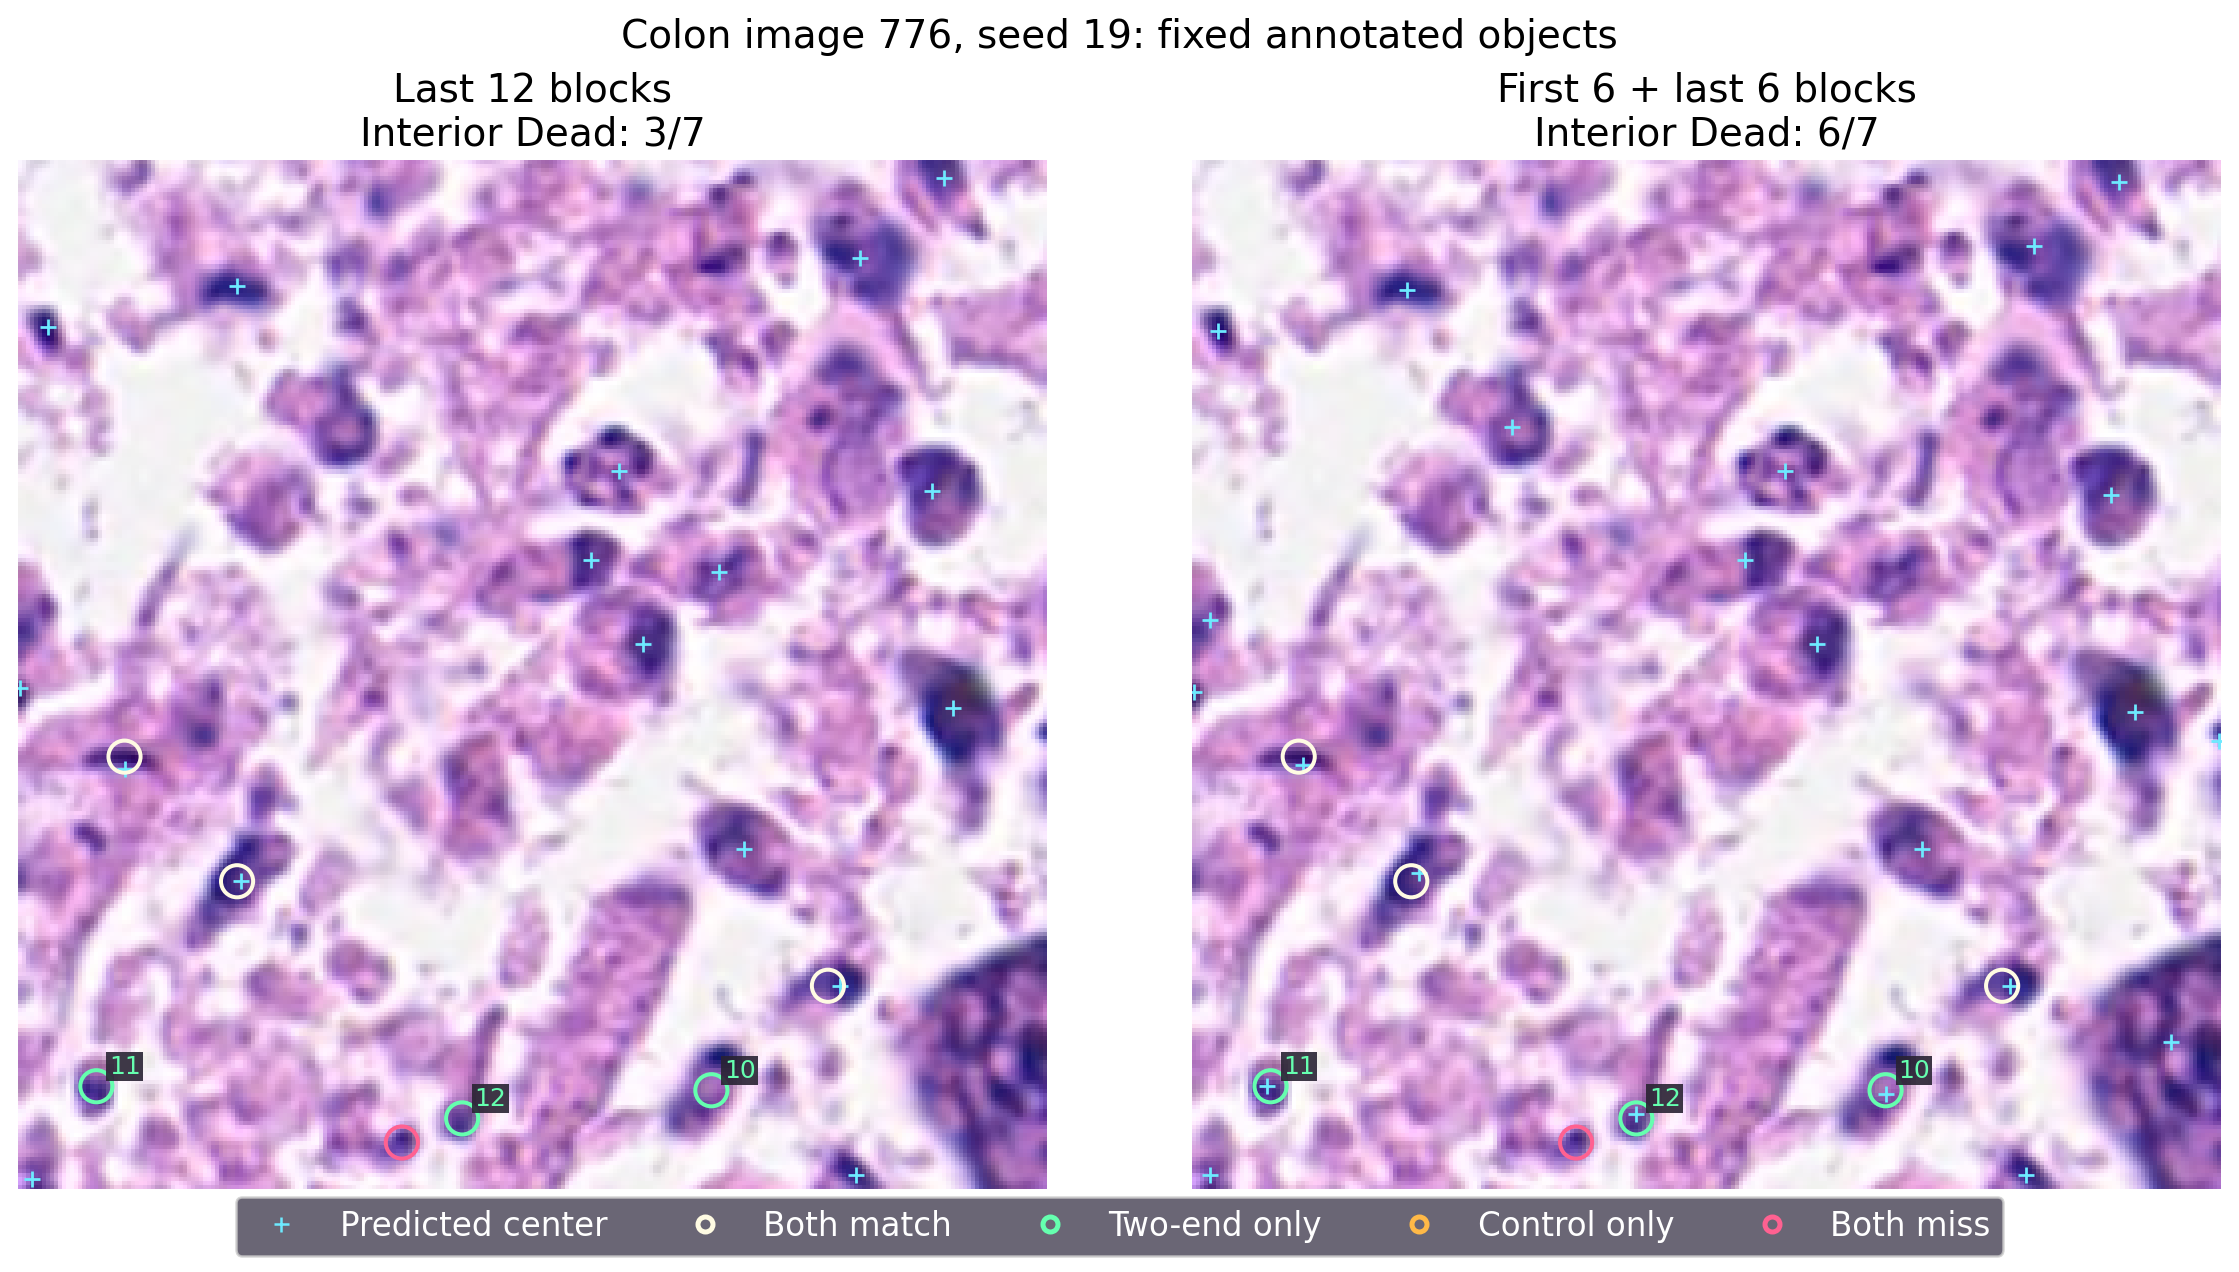
\includegraphics[width=\linewidth,height=.40\textheight,keepaspectratio]{assets/p29_image_776_seed_19.png}
\captionof{figure}{Colon image 776, fixed seed-19 comparison. Seed 19; last-twelve control left, first six and last six intervention right. Cyan crosses mark predictions; white, green, orange and pink circles mark matched by both, intervention only, control only and missed by both}
\raggedright

Colon image 776 changes from 3/7 to 6/7 target matches. Three gained objects lie in the lower tissue strip: object 10 at (231,172), object 11 at (230,19), and object 12 at (238,110). Their nearest decoded-point distances change 41.23 → 1.00, 28.02 → 1.00 and 80.66 → 1.00 pixels. The right panel places predictions close to all three annotations; the control has no decoded point in their immediate neighborhoods. Their visible size and pale appearance vary, and object 12 has area 104 pixels. This is recovery beyond the smallest predefined size bin.

\end{minipage}

\noindent

\begin{minipage}{\linewidth}\centering
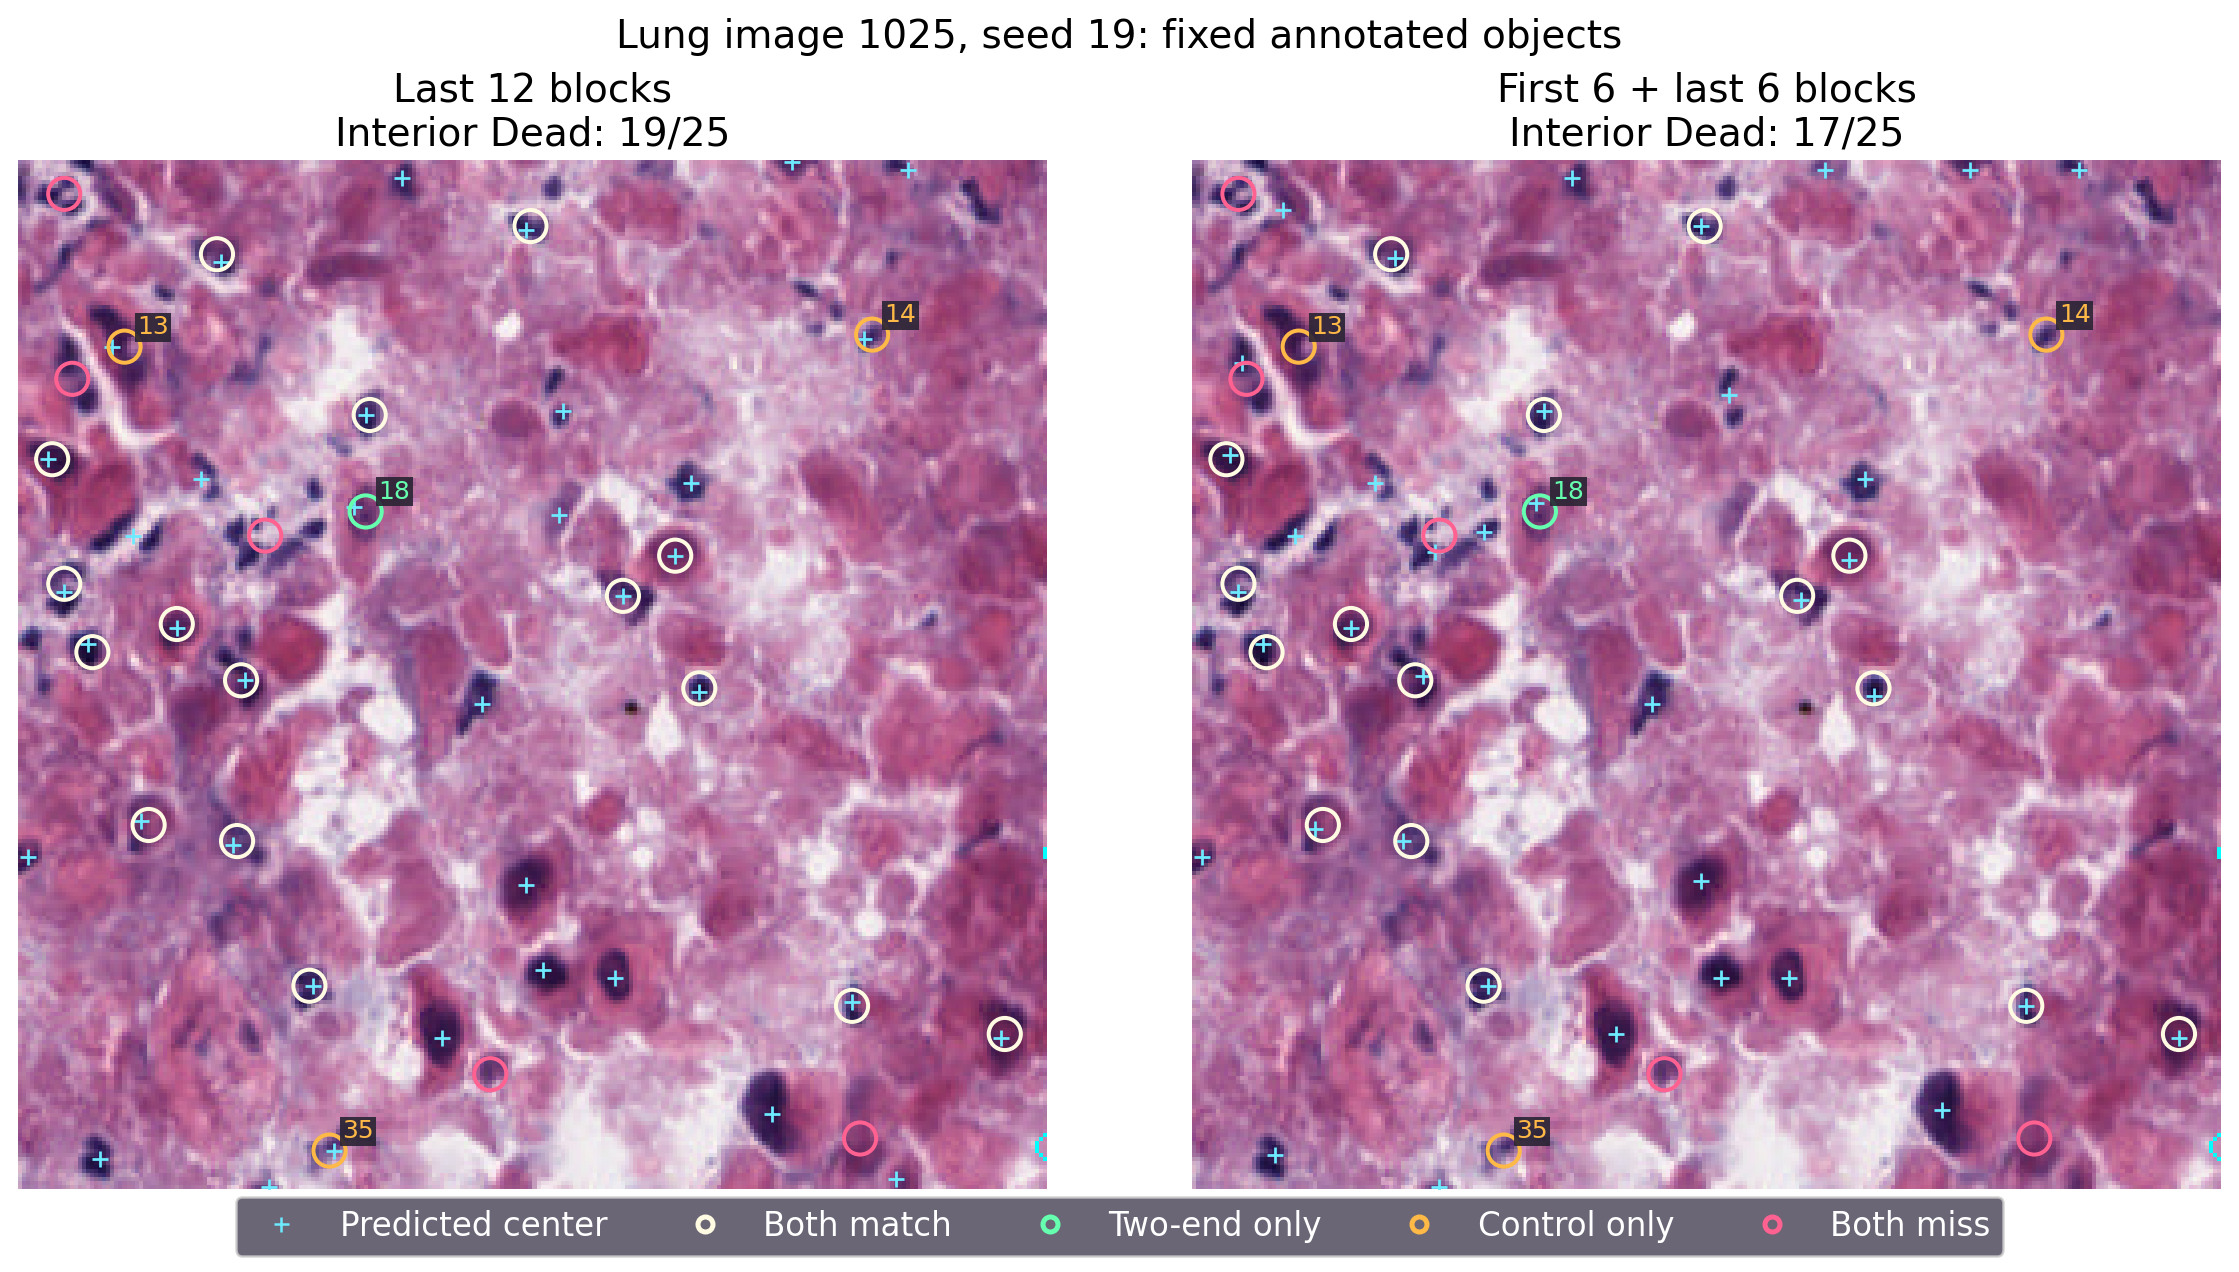
\includegraphics[width=\linewidth,height=.40\textheight,keepaspectratio]{assets/p29_image_1025_seed_19.png}
\captionof{figure}{Lung image 1025: gains alongside lost detections. Seed 19; last-twelve control left, first six and last six intervention right. Cyan crosses mark predictions; white, green, orange and pink circles mark matched by both, intervention only, control only and missed by both}
\raggedright

Lung image 1025 changes from 19/25 to 17/25. Object 18 at (87,86) gains a match as its nearest point moves from 3.16 to 2.24 pixels, crossing the fixed three-pixel matching boundary. Objects 13 at (46,26), 14 at (43,212), and 35 at (246,77) lose matches, with nearest distances 3.00 → 14.56, 2.24 → 41.77 and 1.00 → 18.36. Object 14 has area 31 pixels and is visibly small. The intervention removes useful outputs around these annotations while recovering another object. The full tissue aggregate cannot reveal this exchange.

\end{minipage}

\noindent

\begin{minipage}{\linewidth}\centering
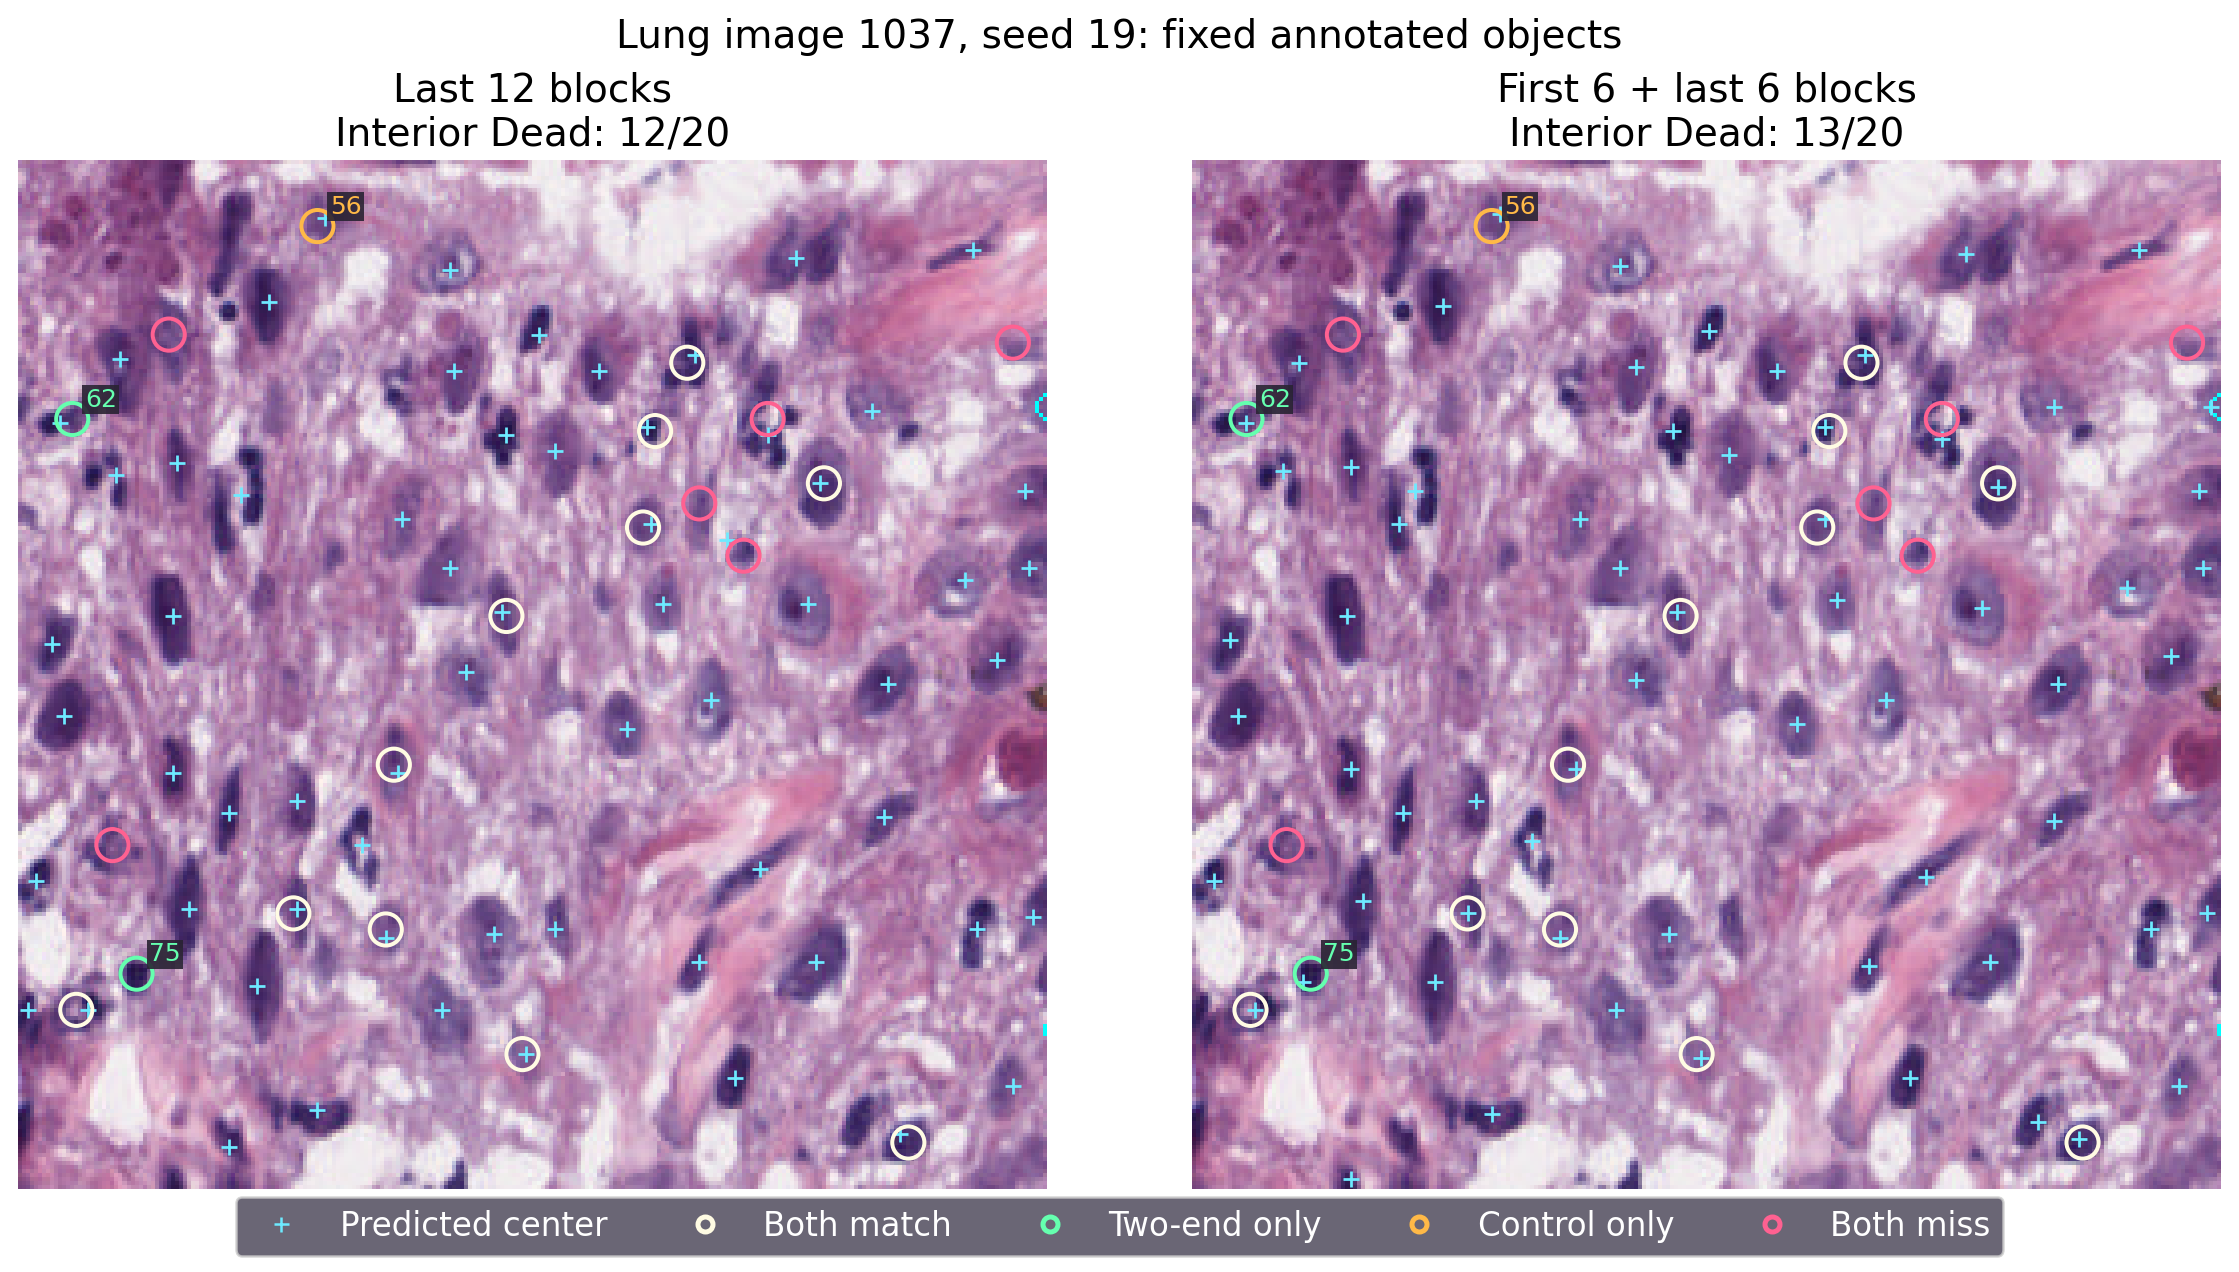
\includegraphics[width=\linewidth,height=.40\textheight,keepaspectratio]{assets/p29_image_1037_seed_19.png}
\captionof{figure}{Lung image 1037: a larger gain and a boundary displacement. Seed 19; last-twelve control left, first six and last six intervention right. Cyan crosses mark predictions; white, green, orange and pink circles mark matched by both, intervention only, control only and missed by both}
\raggedright

Lung image 1037 changes from 12/20 to 13/20. Object 62 at (64,13) gains a match as nearest distance falls 3.16 → 1.00; object 75 at (202,29), area 44 pixels, changes 15.00 → 2.83. Object 56 at (16,74) loses its match after a nearby point shifts from 2.83 to 3.61 pixels. The latter event is a displacement across the matching radius; the former small-object gain places a prediction in a previously uncovered neighborhood.

\end{minipage}

Coordinates establish appearance, disappearance and displacement of
decoded points. Image intensity and tissue context make these events
visible. Attribution to center-score strength, peak suppression or
hidden encoder features requires probability maps or intermediate
measurements; this collection stores original images, annotated centers,
decoded points and one-to-one assignments.

\subsubsection{Seed 1 and consistency across
seeds}\label{seed-1-and-consistency-across-seeds}

{\def\LTcaptype{none} % do not increment counter
\begin{longtable}[]{@{}
  >{\raggedright\arraybackslash}p{(\linewidth - 12\tabcolsep) * \real{0.1111}}
  >{\raggedleft\arraybackslash}p{(\linewidth - 12\tabcolsep) * \real{0.1481}}
  >{\raggedleft\arraybackslash}p{(\linewidth - 12\tabcolsep) * \real{0.1481}}
  >{\raggedleft\arraybackslash}p{(\linewidth - 12\tabcolsep) * \real{0.1481}}
  >{\raggedleft\arraybackslash}p{(\linewidth - 12\tabcolsep) * \real{0.1481}}
  >{\raggedleft\arraybackslash}p{(\linewidth - 12\tabcolsep) * \real{0.1481}}
  >{\raggedleft\arraybackslash}p{(\linewidth - 12\tabcolsep) * \real{0.1481}}@{}}
\toprule\noalign{}
\begin{minipage}[b]{\linewidth}\raggedright
Seed / allocation
\end{minipage} & \begin{minipage}[b]{\linewidth}\raggedleft
Interior Dead
\end{minipage} & \begin{minipage}[b]{\linewidth}\raggedleft
Small Dead
\end{minipage} & \begin{minipage}[b]{\linewidth}\raggedleft
All matched
\end{minipage} & \begin{minipage}[b]{\linewidth}\raggedleft
Recall
\end{minipage} & \begin{minipage}[b]{\linewidth}\raggedleft
Precision
\end{minipage} & \begin{minipage}[b]{\linewidth}\raggedleft
Unmatched
\end{minipage} \\
\midrule\noalign{}
\endhead
\bottomrule\noalign{}
\endlastfoot
1 / last 12 & 67/145 & 7/32 & 7,329/12,250 & 59.83\% & 69.25\% &
3,255 \\
1 / first 6 + last 6 & 80/145 & 11/32 & 7,494/12,250 & 61.18\% & 70.14\%
& 3,191 \\
\end{longtable}
}

Seed 1 adds 13 target matches, with the unchanged tissue-stratified 95\%
bootstrap interval {[}+3.1250,+20.4082{]} percentage points. It emits
101 more predictions and finds 165 more nuclei. Both seeds improve
overall recall, precision and small-Dead coverage, while training
coverage falls. The final Dead recall and precision were below the
original 60\% and 75\% criteria in both seeds. The observed means of the
within-seed changes are 10.0 percentage points for Dead recall, 1.83
points for all-nucleus recall and 1.06 points for precision; the same
images occur in both seeds, so these means summarize the paired outcomes
without doubling the image sample size.

Seed 1 gains on five images, loses one and is unchanged on five. Lung
contributes +6, cervix +5, colon +1 and esophagus +1. Lung image 1038
contributes +4 in seed 1 and +5 in seed 19. Cervix 1756 contributes
+5/+2. Colon 1482 instead changes 11/49 → 10/49 in seed 1 and 13/49 →
13/49 in seed 19: 39/36 target objects remain missed in this
concentrated image. Lung 1025 reverses direction between seeds, −2/+2.
Both seeds improve in the aggregate, but their gains are distributed
differently. Removing any single positive image leaves gains of
6.15--14.58 percentage points in seed 1, alongside 8.03--16.67 in seed
19.

Training recall falls from 97.80\% to 95.43\%, and training Dead matches
from 624/656 to 606/656. Recorded training time is 4.0143 versus 6.7220
hours; checkpoint time is 238.77 versus 2,116.75 seconds. The seed-1
intervention was exposed to prolonged Lustre delays, and its application
completion time is 10.1409 hours. These elapsed timings include stalls
and provide a resource record, while the seed-19 21.24\% training
increase is the cleaner same-round cost comparison. GPU peaks are the
same across seeds: about 4.05 versus 4.84 GiB.

\subsubsection{Fixed objects that replicate, reverse or exchange across
seeds}\label{fixed-objects-that-replicate-reverse-or-exchange-across-seeds}

The fixed eight images in seed 1 retain 29 objects, gain 7, lose 3 and
miss 14 in both arms, for net +4 out of 53. Together with seed 19's
retained 30, gained 6, lost 4 and jointly missed 13, they expose local
changes behind the aggregate improvement.

\noindent

\begin{minipage}{\linewidth}\centering
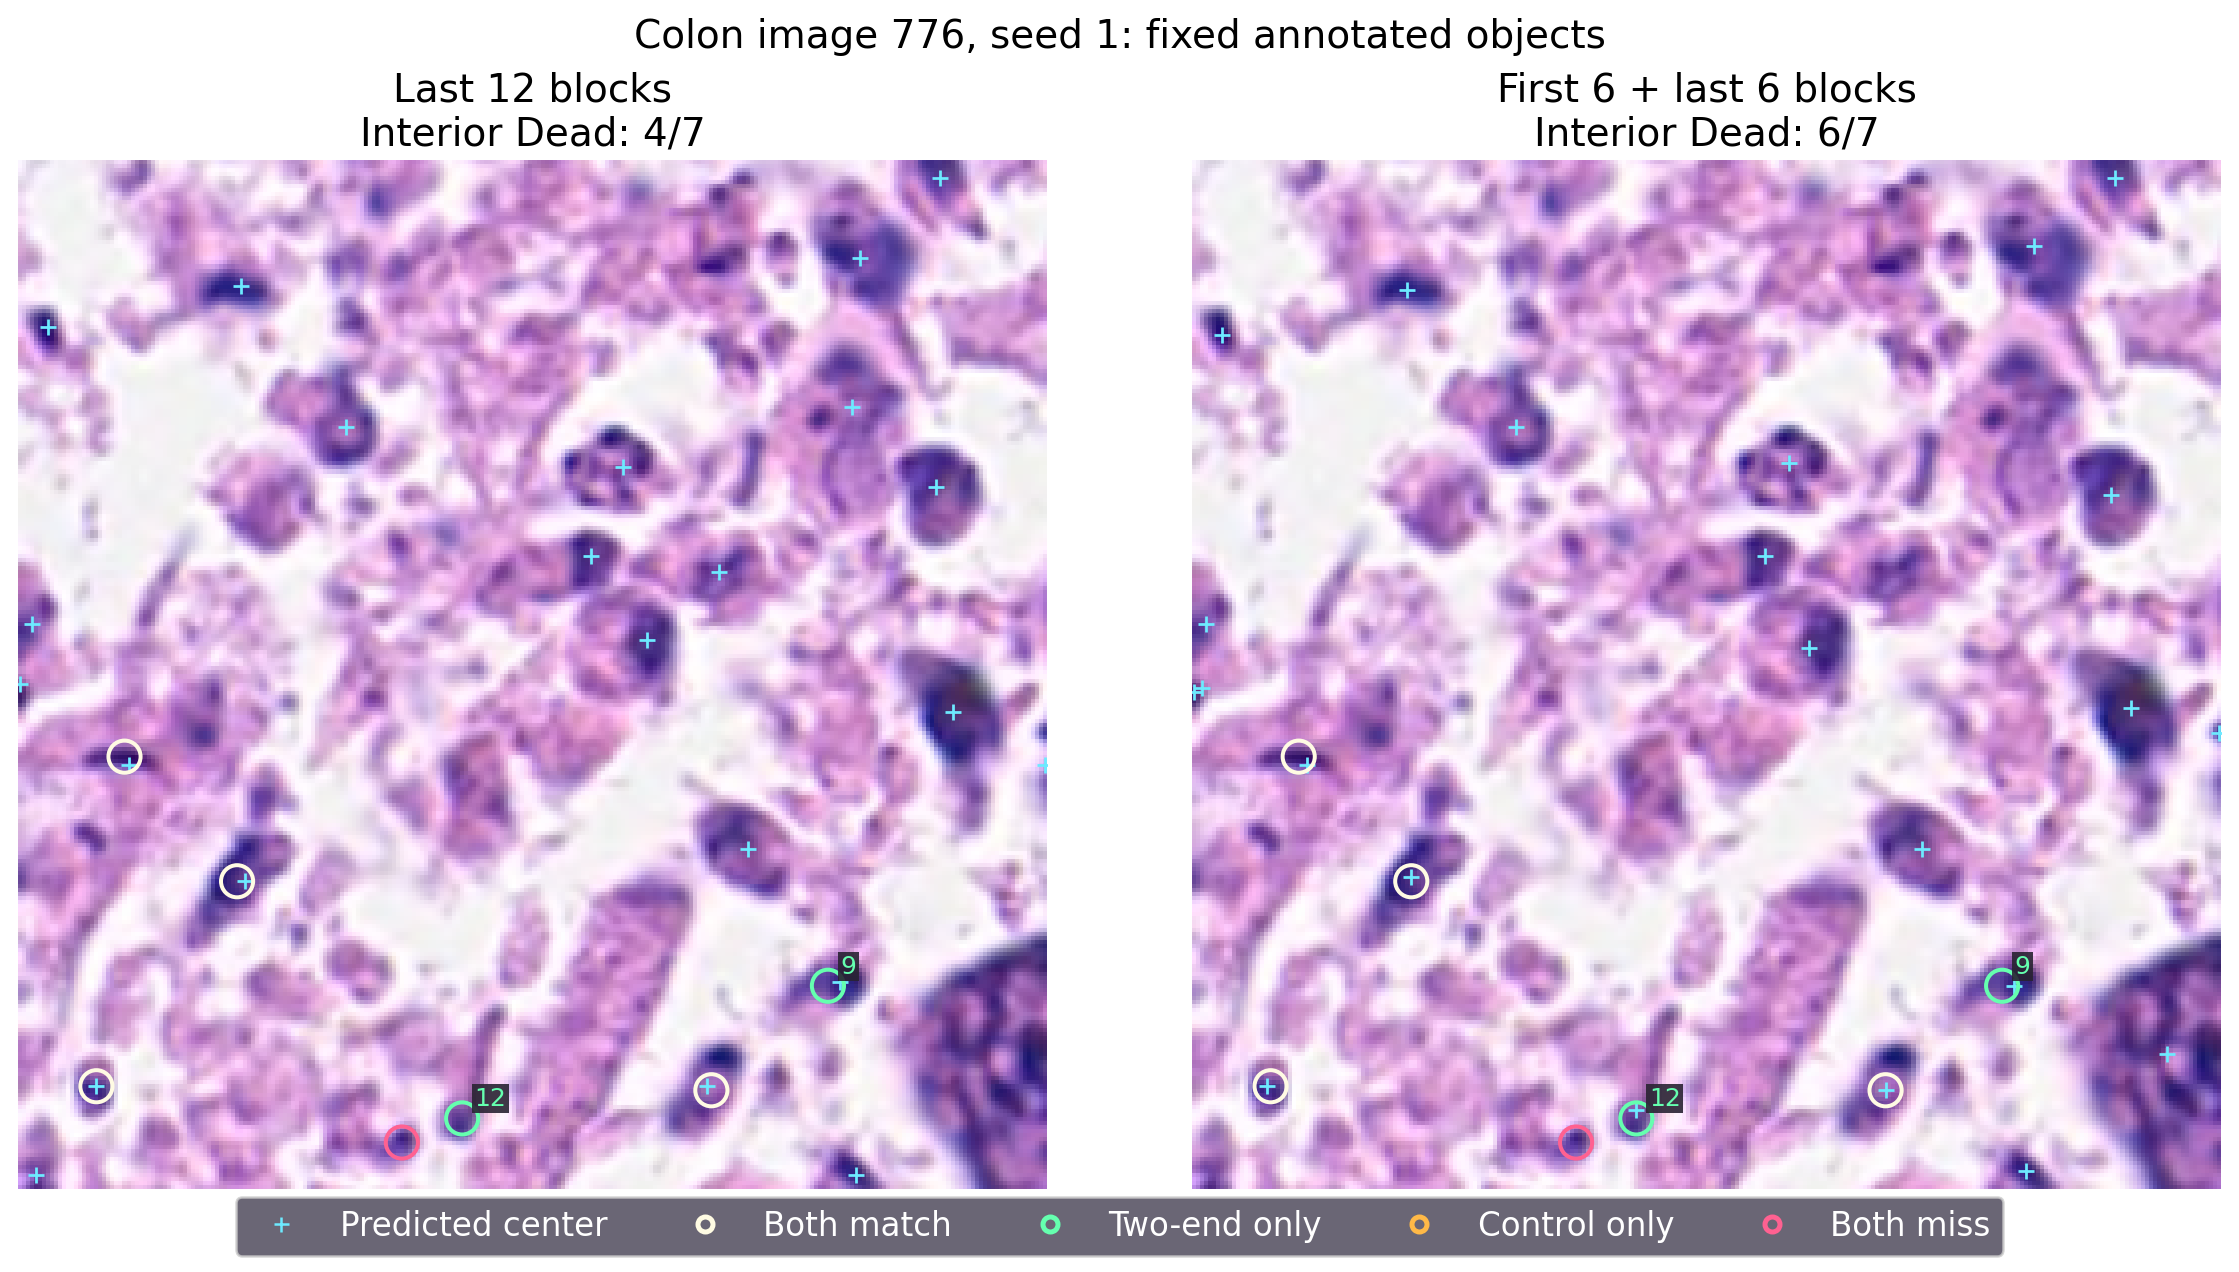
\includegraphics[width=\linewidth,height=.40\textheight,keepaspectratio]{assets/p29_image_776_seed_1.png}
\captionof{figure}{Seed 1, colon 776. Seed 1; last-twelve control left, first six and last six intervention right. Cyan crosses mark predictions; white, green, orange and pink circles mark matched by both, intervention only, control only and missed by both}
\raggedright

Colon 776 improves 4/7 → 6/7. Object 12 at (238,110), area 104, is recovered in both seeds: its nearest prediction moves 61.52 → 2.00 pixels in seed 1 and 80.66 → 1.00 in seed 19. This shared recovery provides a concrete repeatable example at the same annotation. Seed 1 also gains object 9 at (205,201), area 191, as its distance crosses 3.16 → 3.00 pixels. Seed 19 instead gains objects 10 and 11 in the lower strip, demonstrating that the same total benefit can involve different nuclei.

\end{minipage}

\noindent

\begin{minipage}{\linewidth}\centering
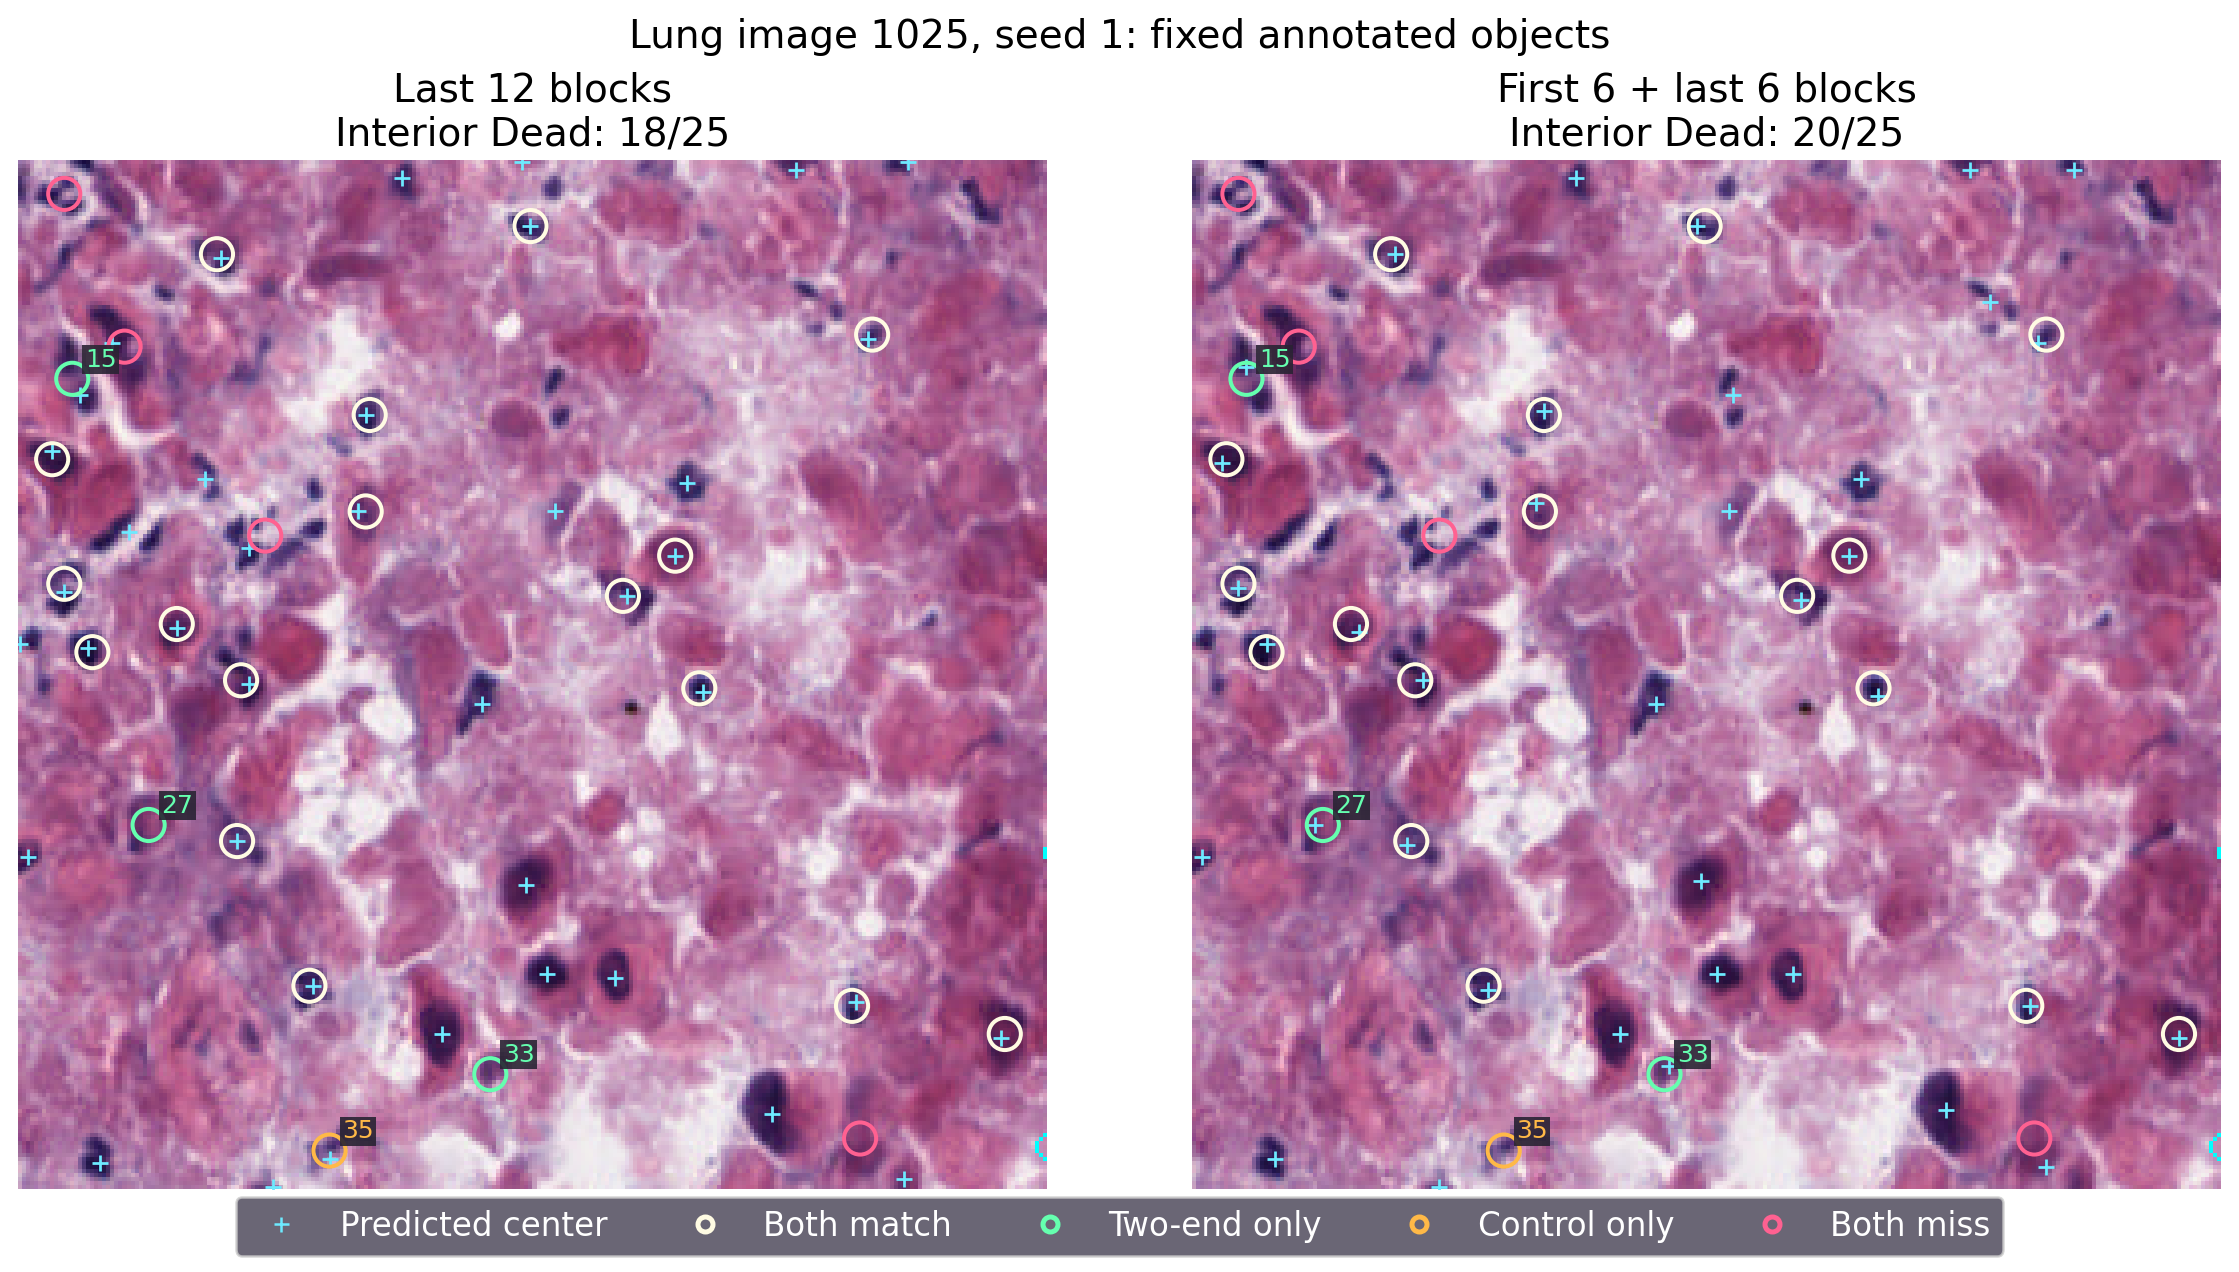
\includegraphics[width=\linewidth,height=.40\textheight,keepaspectratio]{assets/p29_image_1025_seed_1.png}
\captionof{figure}{Seed 1, lung 1025. Seed 1; last-twelve control left, first six and last six intervention right. Cyan crosses mark predictions; white, green, orange and pink circles mark matched by both, intervention only, control only and missed by both}
\raggedright

Lung 1025 improves 18/25 → 20/25 in seed 1. Objects 15 (54,13), 27 (165,32) and 33 (227,117) are gained, with distances 4.47 → 3.00, 22.36 → 2.00 and 15.62 → 2.24 pixels. Object 33 has area 52, placing it in the predefined small-object subset. Object 35 (246,77), area 68, is lost in both seeds: 2.00 → 18.36 in seed 1 and 1.00 → 18.36 in seed 19. That repeated loss coexists with the positive tissue-level aggregate.

\end{minipage}

\noindent

\begin{minipage}{\linewidth}\centering
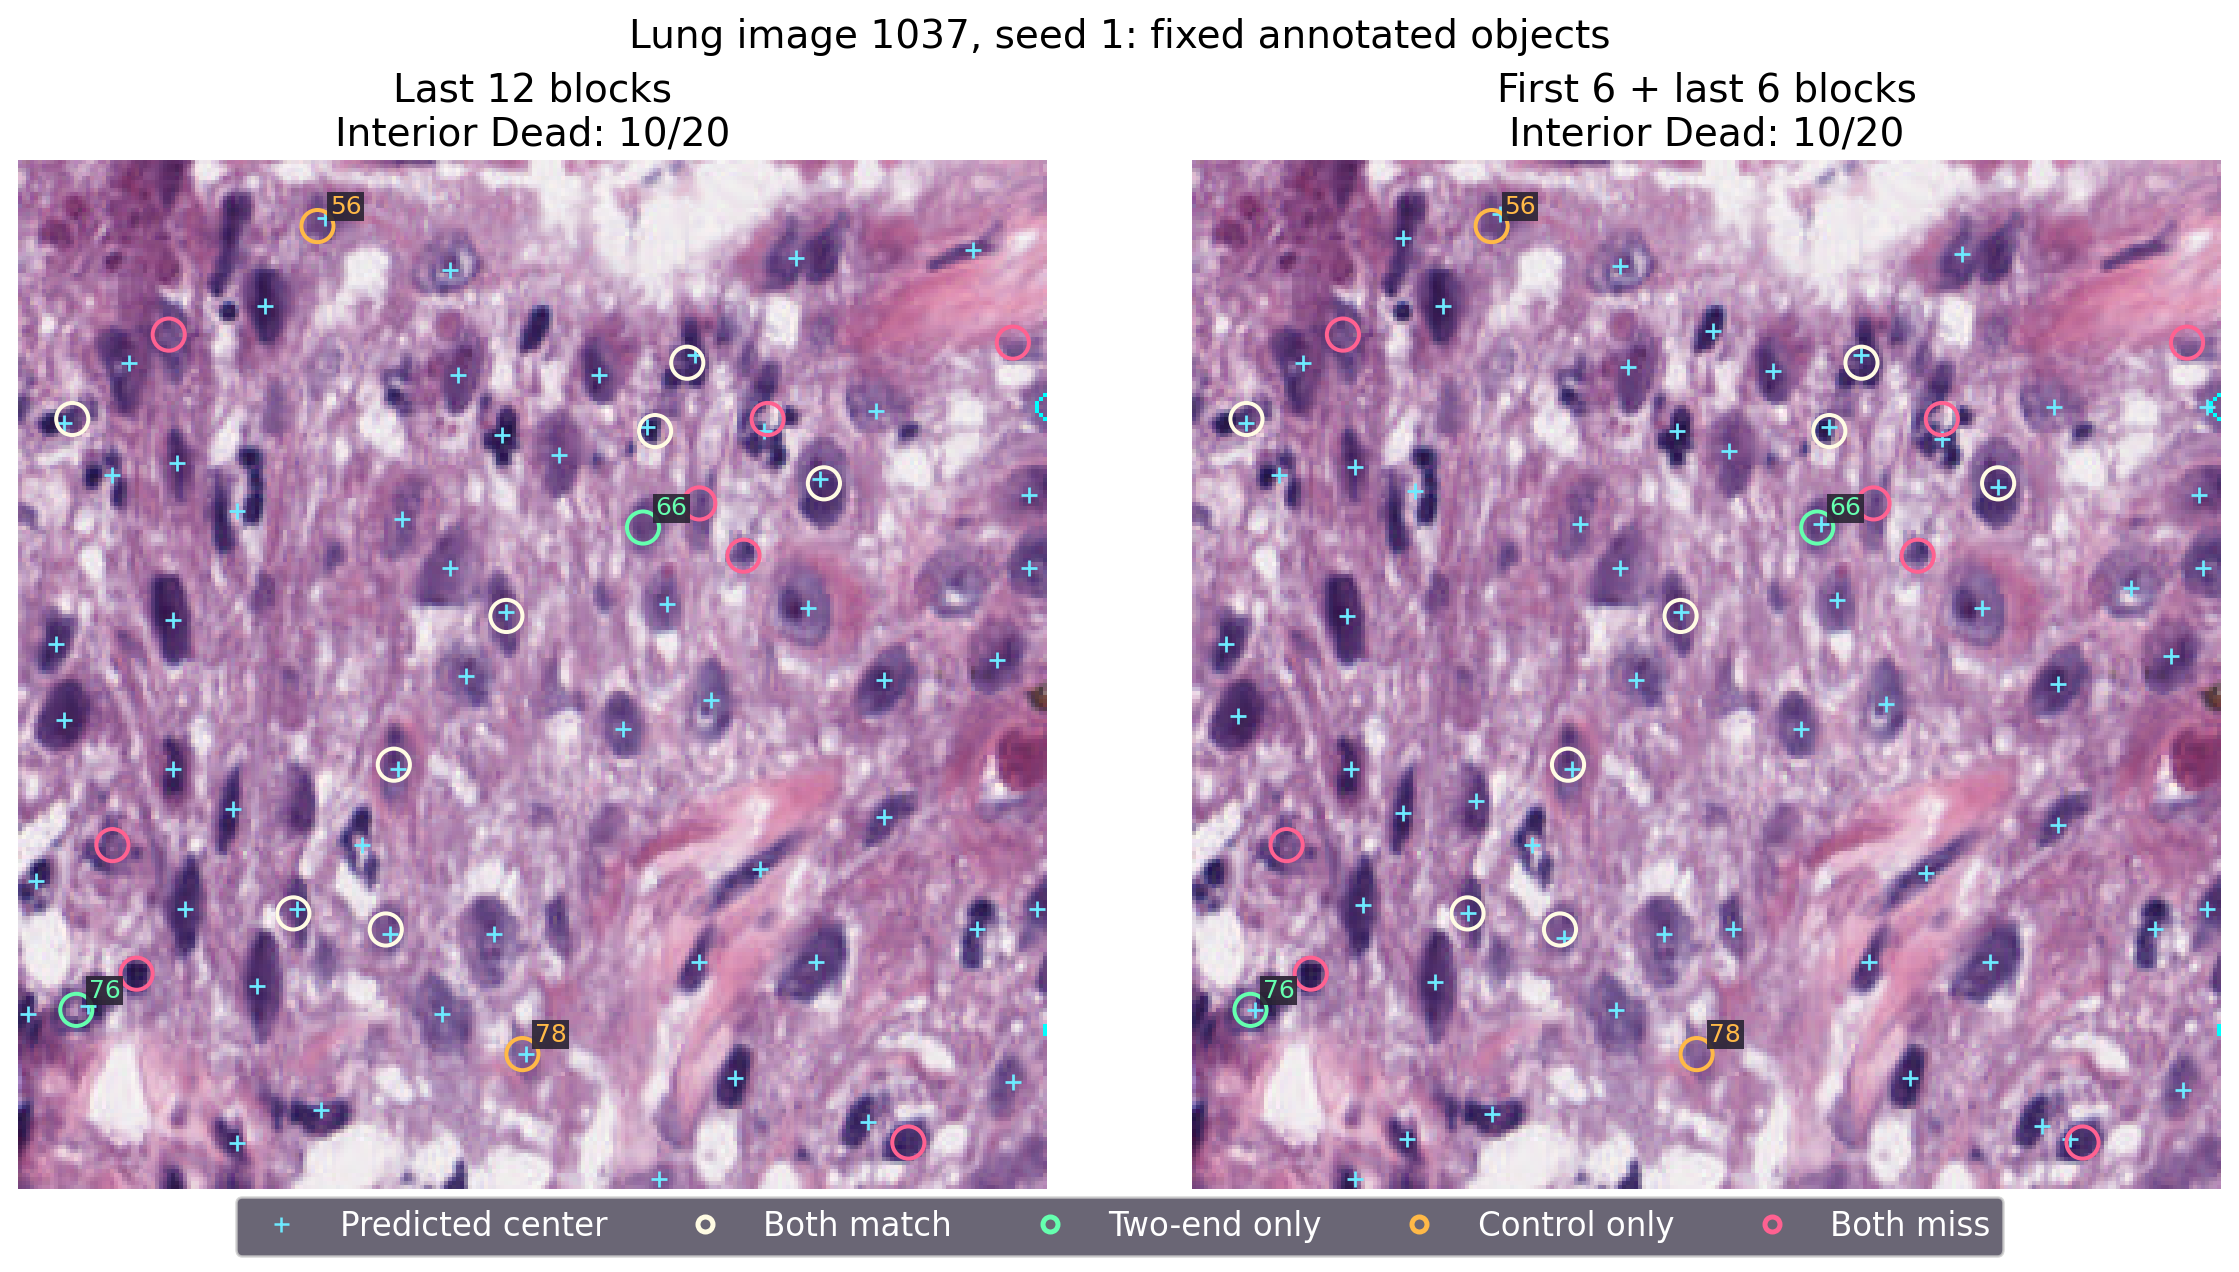
\includegraphics[width=\linewidth,height=.40\textheight,keepaspectratio]{assets/p29_image_1037_seed_1.png}
\captionof{figure}{Seed 1, lung 1037. Seed 1; last-twelve control left, first six and last six intervention right. Cyan crosses mark predictions; white, green, orange and pink circles mark matched by both, intervention only, control only and missed by both}
\raggedright

Lung 1037 stays at 10/20 in seed 1, exchanging two gains and two losses. Objects 66 (91,155) and 76 (211,14) gain predictions at distances 19.92 → 1.41 and 3.16 → 1.00; objects 56 (16,74) and 78 (222,125) lose matches at 2.83 → 3.61 and 1.00 → 22.83. Object 56 crosses the identical boundary in both seeds. An unchanged image count can therefore conceal repeated localization loss plus compensating recovery elsewhere. All object distances, original centers and one-to-one assignments are included in the CSV and raw coordinate JSONs.

\end{minipage}

\subsection{P30: updating the middle twelve
blocks}\label{p30-updating-the-middle-twelve-blocks}

P30 updates blocks 6--17 instead of 12--23, numbered from zero,
retaining the same encoder and head parameter counts, rates and training
schedule. All four tasks in array 55746187 completed successfully, each
with 130 consecutive epochs and final development evaluation. Their
combined scheduler duration is 17.4389 GPU hours.

{\def\LTcaptype{none} % do not increment counter
\begin{longtable}[]{@{}
  >{\raggedright\arraybackslash}p{(\linewidth - 12\tabcolsep) * \real{0.1111}}
  >{\raggedleft\arraybackslash}p{(\linewidth - 12\tabcolsep) * \real{0.1481}}
  >{\raggedleft\arraybackslash}p{(\linewidth - 12\tabcolsep) * \real{0.1481}}
  >{\raggedleft\arraybackslash}p{(\linewidth - 12\tabcolsep) * \real{0.1481}}
  >{\raggedleft\arraybackslash}p{(\linewidth - 12\tabcolsep) * \real{0.1481}}
  >{\raggedleft\arraybackslash}p{(\linewidth - 12\tabcolsep) * \real{0.1481}}
  >{\raggedleft\arraybackslash}p{(\linewidth - 12\tabcolsep) * \real{0.1481}}@{}}
\toprule\noalign{}
\begin{minipage}[b]{\linewidth}\raggedright
Run
\end{minipage} & \begin{minipage}[b]{\linewidth}\raggedleft
Interior Dead
\end{minipage} & \begin{minipage}[b]{\linewidth}\raggedleft
Small Dead
\end{minipage} & \begin{minipage}[b]{\linewidth}\raggedleft
All matches
\end{minipage} & \begin{minipage}[b]{\linewidth}\raggedleft
Predictions
\end{minipage} & \begin{minipage}[b]{\linewidth}\raggedleft
Recall
\end{minipage} & \begin{minipage}[b]{\linewidth}\raggedleft
Precision
\end{minipage} \\
\midrule\noalign{}
\endhead
\bottomrule\noalign{}
\endlastfoot
Seed 19, last twelve & 71/145 & 9/32 & 7,246 & 10,539 & 59.151\% &
68.754\% \\
Seed 19, middle twelve & 78/145 & 14/32 & 7,894 & 10,972 & 64.441\% &
71.947\% \\
Seed 1, last twelve & 64/145 & 8/32 & 7,338 & 10,647 & 59.902\% &
68.921\% \\
Seed 1, middle twelve & 79/145 & 13/32 & 7,854 & 10,909 & 64.114\% &
71.996\% \\
\end{longtable}
}

The intervention emits 433/262 more predictions but finds 648/516 more
nuclei, reducing unmatched predictions by 215/254. Overall recall
improves by 5.2898/4.2122 percentage points and precision by
3.1926/3.0748 points. Small-Dead coverage gains five objects in each
seed. Interior Dead recall improves by 4.8276/10.3448 points; its
original 95\% intervals are {[}−0.9091,+9.6552{]} and
{[}+1.8987,+18.3673{]} points.

The original criteria included a final Dead recall of at least 60\%,
precision of at least 75\%, and a prespecified improvement relative to
the control. The observed Dead recall was 53.79\%/54.48\% and precision
was 71.95\%/72.00\%; the fixed middle-twelve comparison was completed
under the original rule.

\subsubsection{P30 tissue distribution and training
cost}\label{p30-tissue-distribution-and-training-cost}

Lung contributes +5/+9 and colon +3/+6; cervix loses one match in each
seed. Lung 1037 gains four/six, lung 1038 gains two/four and colon 1482
gains three/five. Lung 1025 loses one in each seed. Colon 1482 ends at
17/49 and 16/49 target matches, leaving 32/33 target objects uncovered.
Its positive change reduces a concentrated miss burden while retaining
substantial remaining work.

Seed 19 has three positive, two negative and six unchanged target-image
counts; seed 1 has five positive, two negative and four unchanged.
Removing one positive image at a time as a descriptive sensitivity
calculation yields gain ranges of 2.40--6.67 and 7.20--13.33 percentage
points. Both signs survive any single-image omission, while the original
bootstrap reflects resampling uncertainty over the full fixed image set.

Training all-nucleus recall changes 97.85\% → 97.10\% and 98.05\% →
97.12\%. Pure training lasts 14,457.50 versus 15,957.59 seconds in seed
19, and 14,509.86 versus 15,957.90 in seed 1: increases of approximately
10.4\% and 10.0\%. Peak allocated training memory rises from 4.05 to
4.44 GiB. Middle-depth adaptation thus delivers broad development gains
at a moderate measured cost without increasing trainable capacity. The
changed path through frozen blocks affects computation even when
parameter counts match.

\subsubsection{P30 fixed objects: recovery, loss and seed
variation}\label{p30-fixed-objects-recovery-loss-and-seed-variation}

The eight predetermined development examples contain 53 interior Dead
annotations. Seed 19 retains 29, gains eight, loses five and misses
eleven in both arms; seed 1 retains 26, gains eleven, loses five and
misses eleven in both. Their net gains are +3/+6. Green rings mark
intervention-only matches, orange rings control-only matches, white
shared matches and pink shared misses; cyan crosses show decoded
predictions. All object indices and row,column positions accompany the
report in CSV and coordinate JSON files.

\noindent

\begin{minipage}{\linewidth}\centering
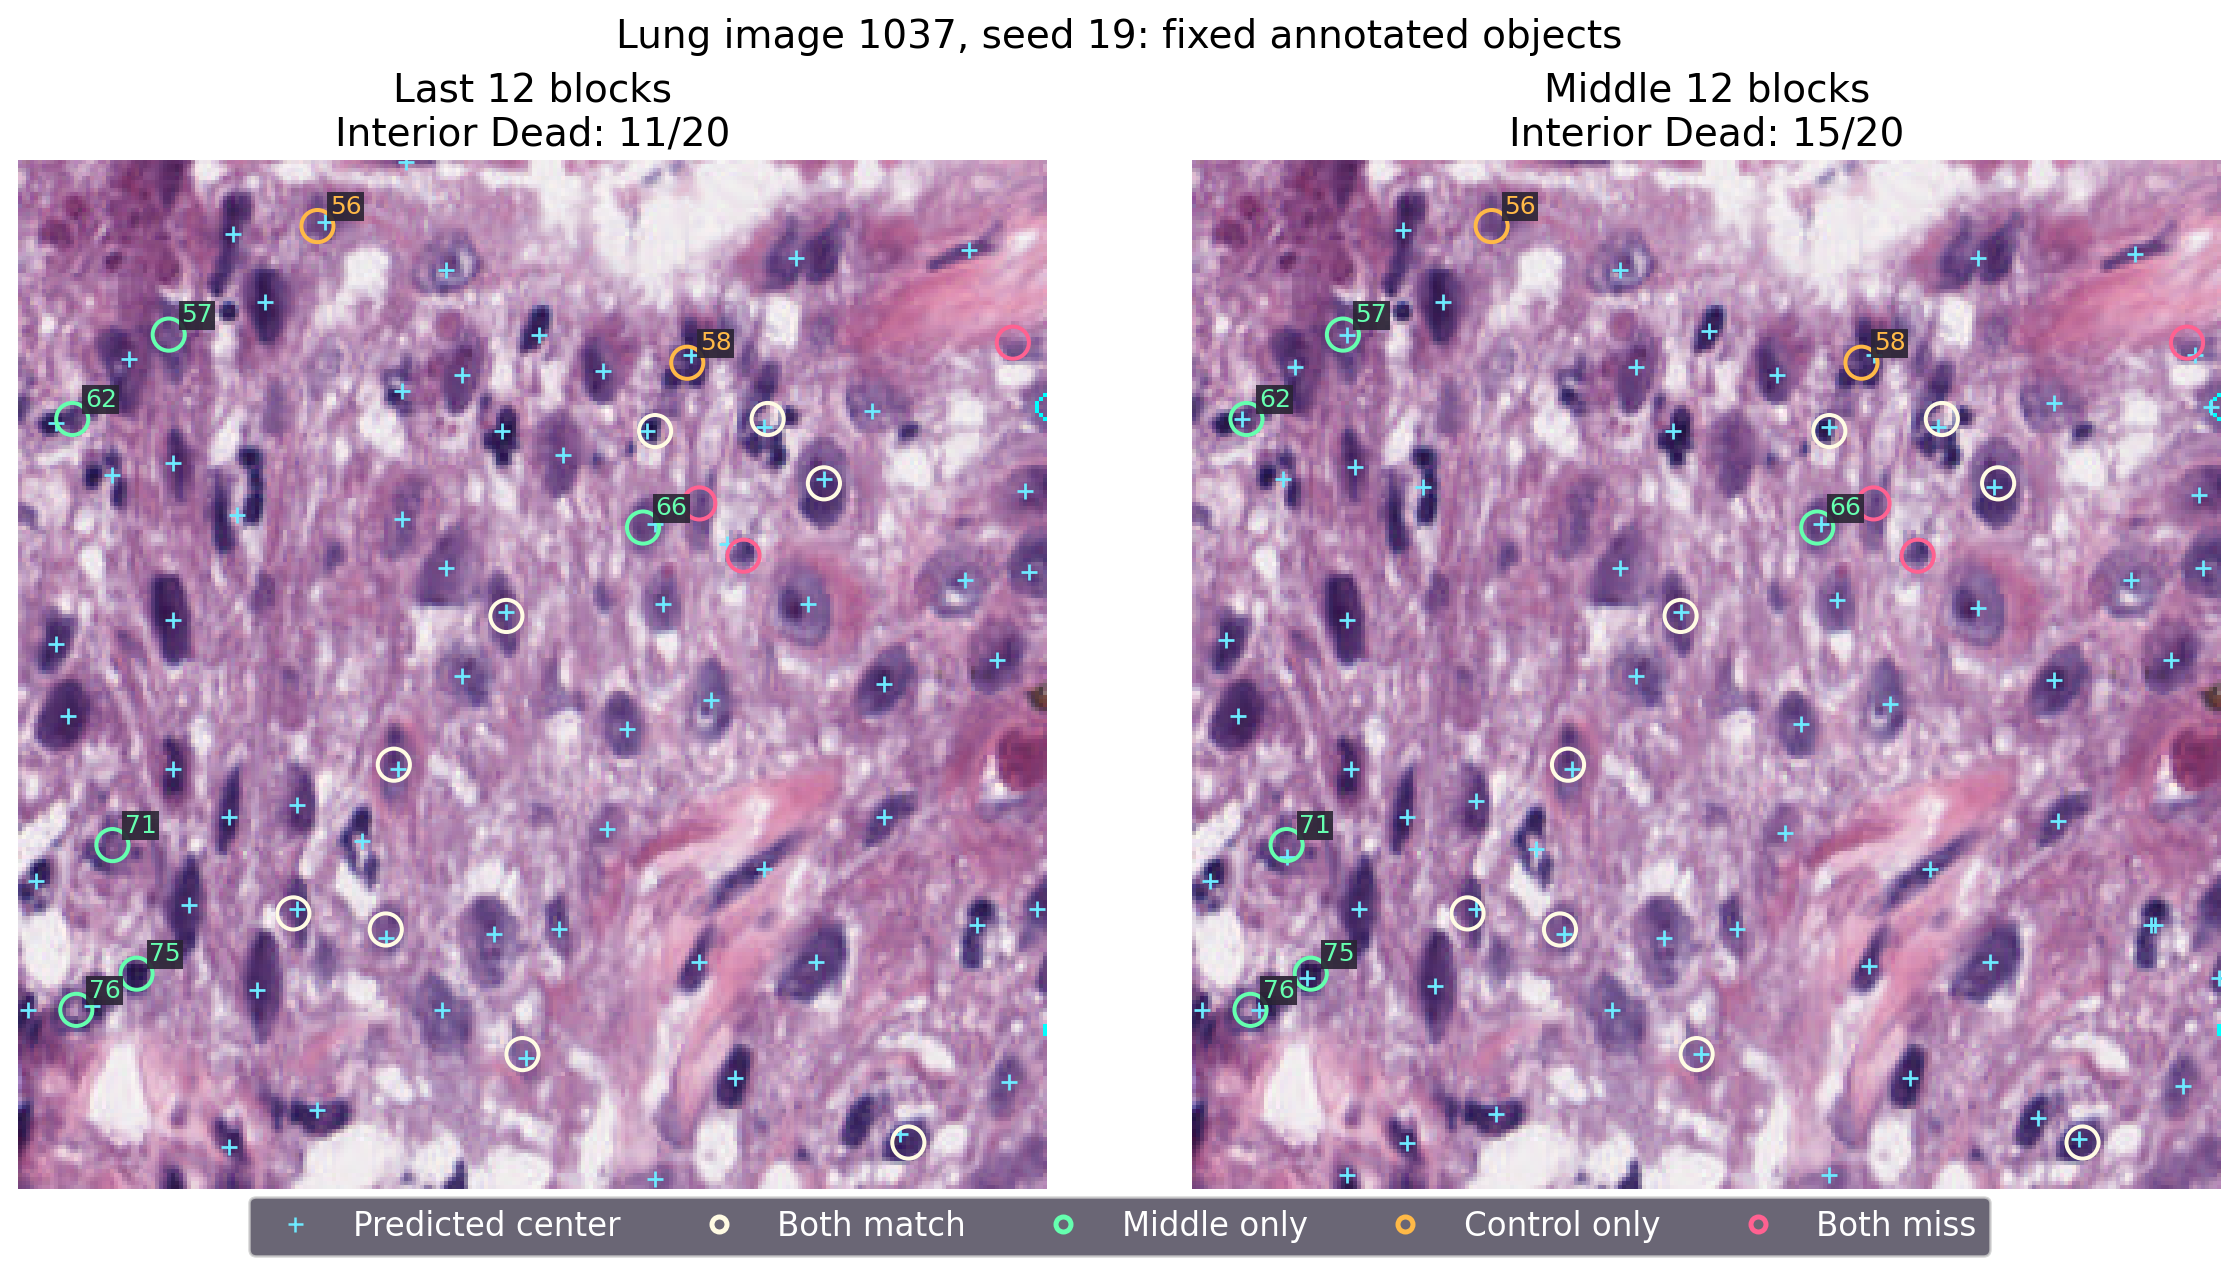
\includegraphics[width=\linewidth,height=.40\textheight,keepaspectratio]{assets/p30_image_1037_seed_19.png}
\captionof{figure}{P30, lung image 1037, seed 19: six gains and two losses. Seed 19; last-twelve control left, middle twelve intervention right. Cyan crosses mark predictions; white, green, orange and pink circles mark matched by both, intervention only, control only and missed by both}
\raggedright

Lung 1037 changes 11/20 → 15/20. Object 75 at (202,29), area 44, gains a point, 13.60 → 1.41 pixels, in the same lower-left neighborhood recovered by several earlier configurations. Object 57 at (43,37), a pale rounded nucleus beside darker neighboring tissue, changes 11.66 → 1.00. Objects 62, 66, 71 and 76 also gain matches. Object 56 (16,74) loses its nearby prediction, 2.24 → 22.02; object 58 (50,166) changes 2.24 → 3.61. The latter is a boundary crossing, whereas the former leaves a much larger gap to the nearest point.

\end{minipage}

\noindent

\begin{minipage}{\linewidth}\centering
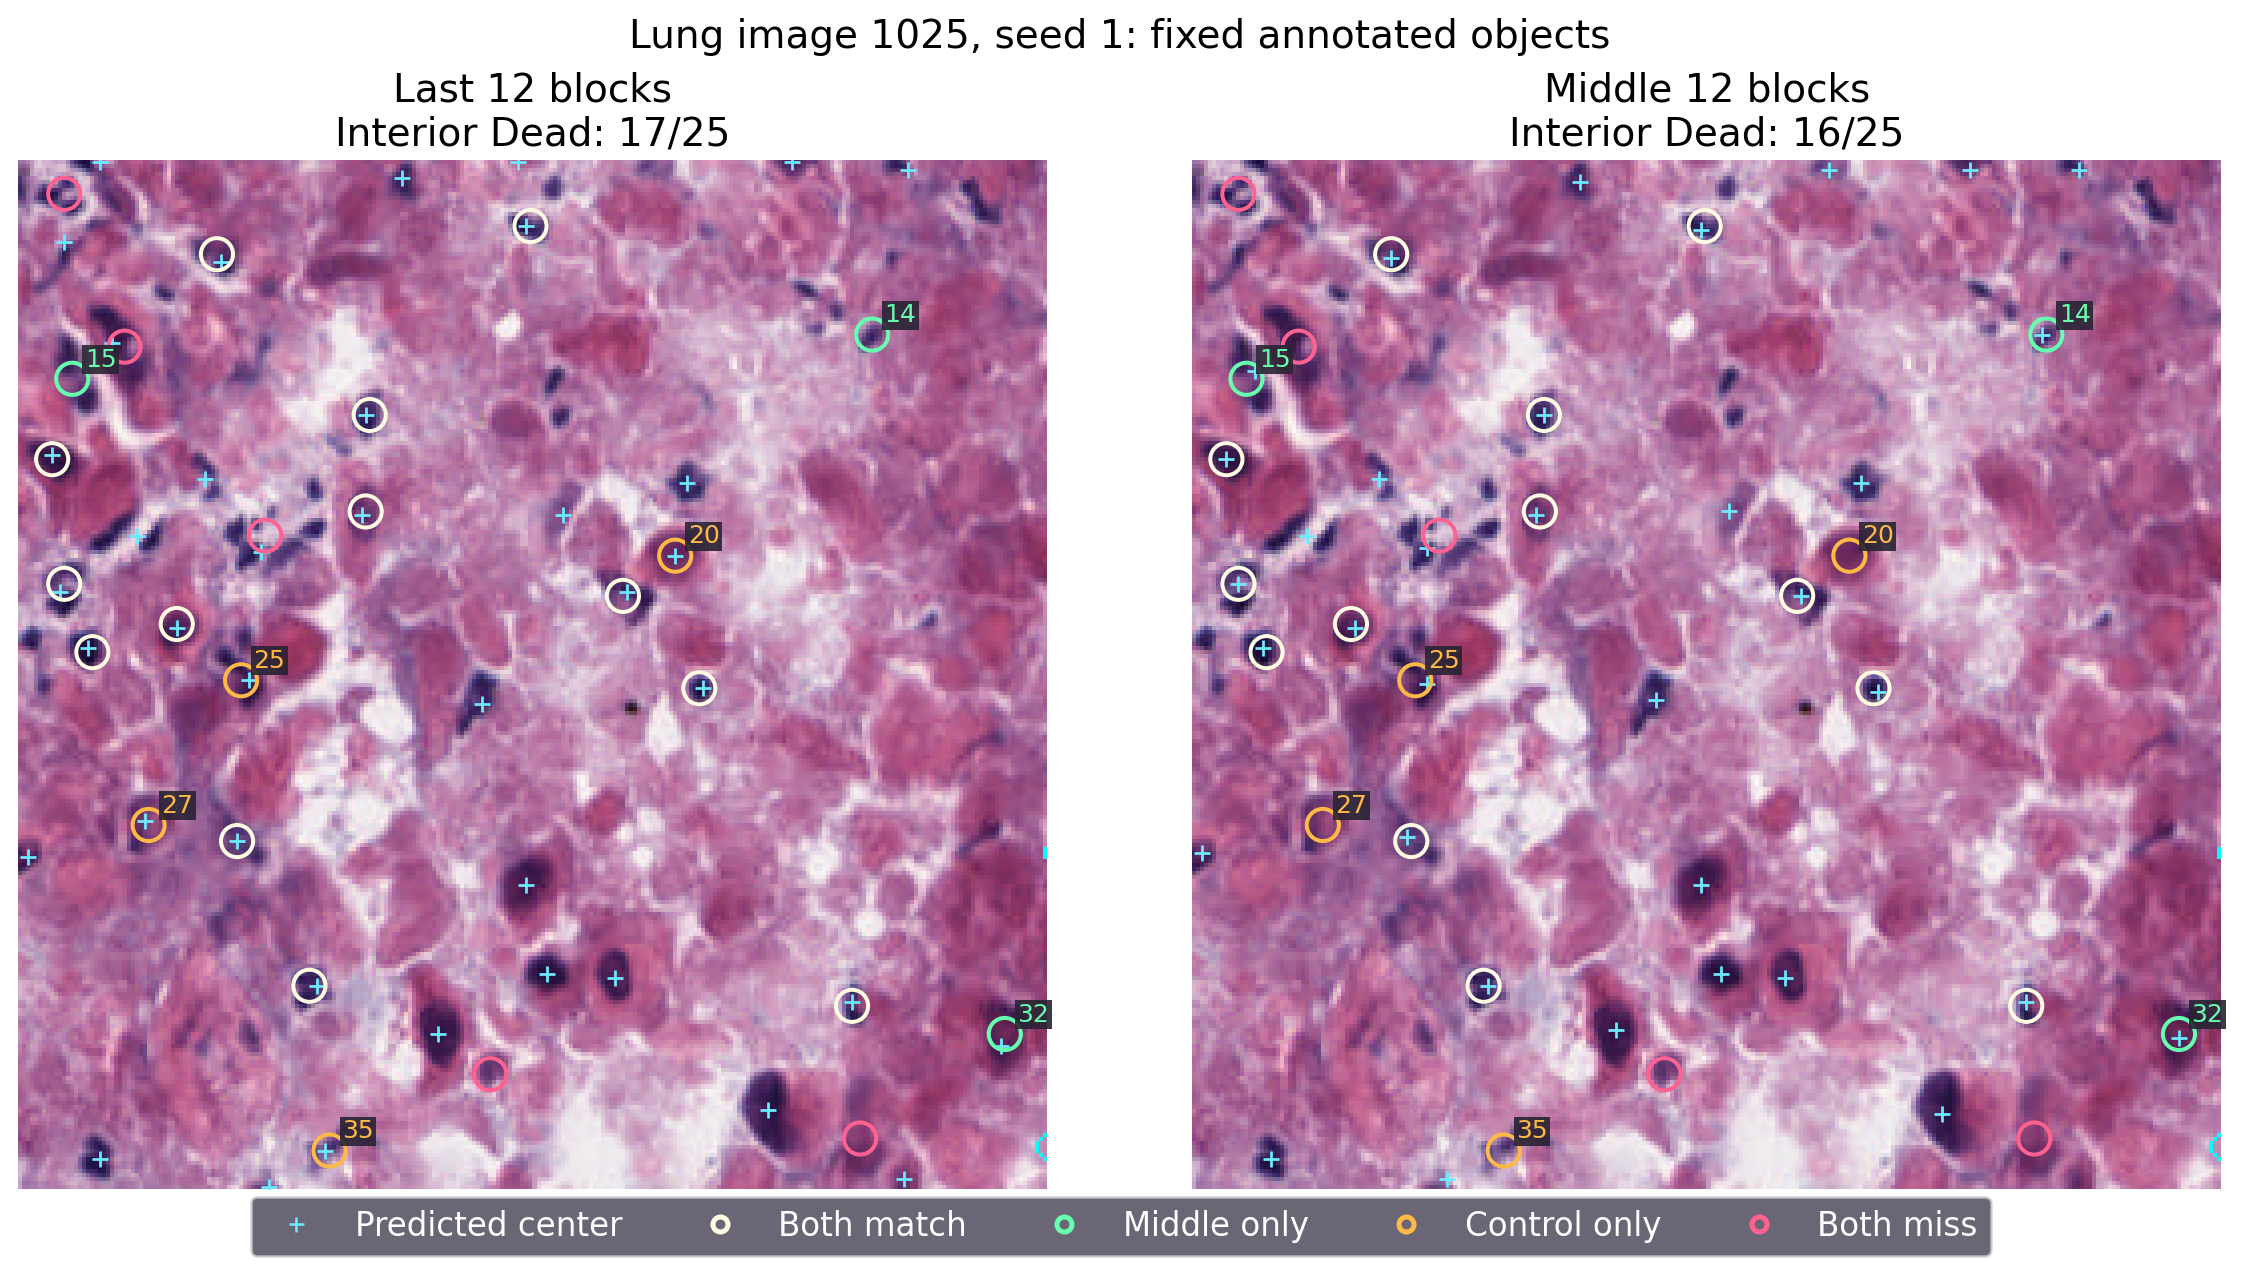
\includegraphics[width=\linewidth,height=.40\textheight,keepaspectratio]{assets/p30_image_1025_seed_1.png}
\captionof{figure}{P30, lung image 1025, seed 1: a recovered small nucleus alongside four losses. Seed 1; last-twelve control left, middle twelve intervention right. Cyan crosses mark predictions; white, green, orange and pink circles mark matched by both, intervention only, control only and missed by both}
\raggedright

Lung 1025 changes 17/25 → 16/25 through three gains and four losses. Object 14 at (43,212), area 31, is recovered at 41.98 → 1.00 pixels. Object 15 (54,13) changes 13.45 → 2.83 and object 32 (217,245) crosses 3.16 → 1.00. Objects 20 (98,163), 27 (165,32) and 35 (246,77) lose nearby outputs, leaving distances 15.62, 21.21 and 15.65 pixels. Object 25 (129,55) changes 2.00 → 3.16 and narrowly crosses the matching radius. In seed 19, the same small object 14 reverses: 2.00 → 41.98 pixels. This annotation gives a concrete example of optimization-seed sensitivity within a tissue image whose net loss repeats.

\end{minipage}

\noindent

\begin{minipage}{\linewidth}\centering
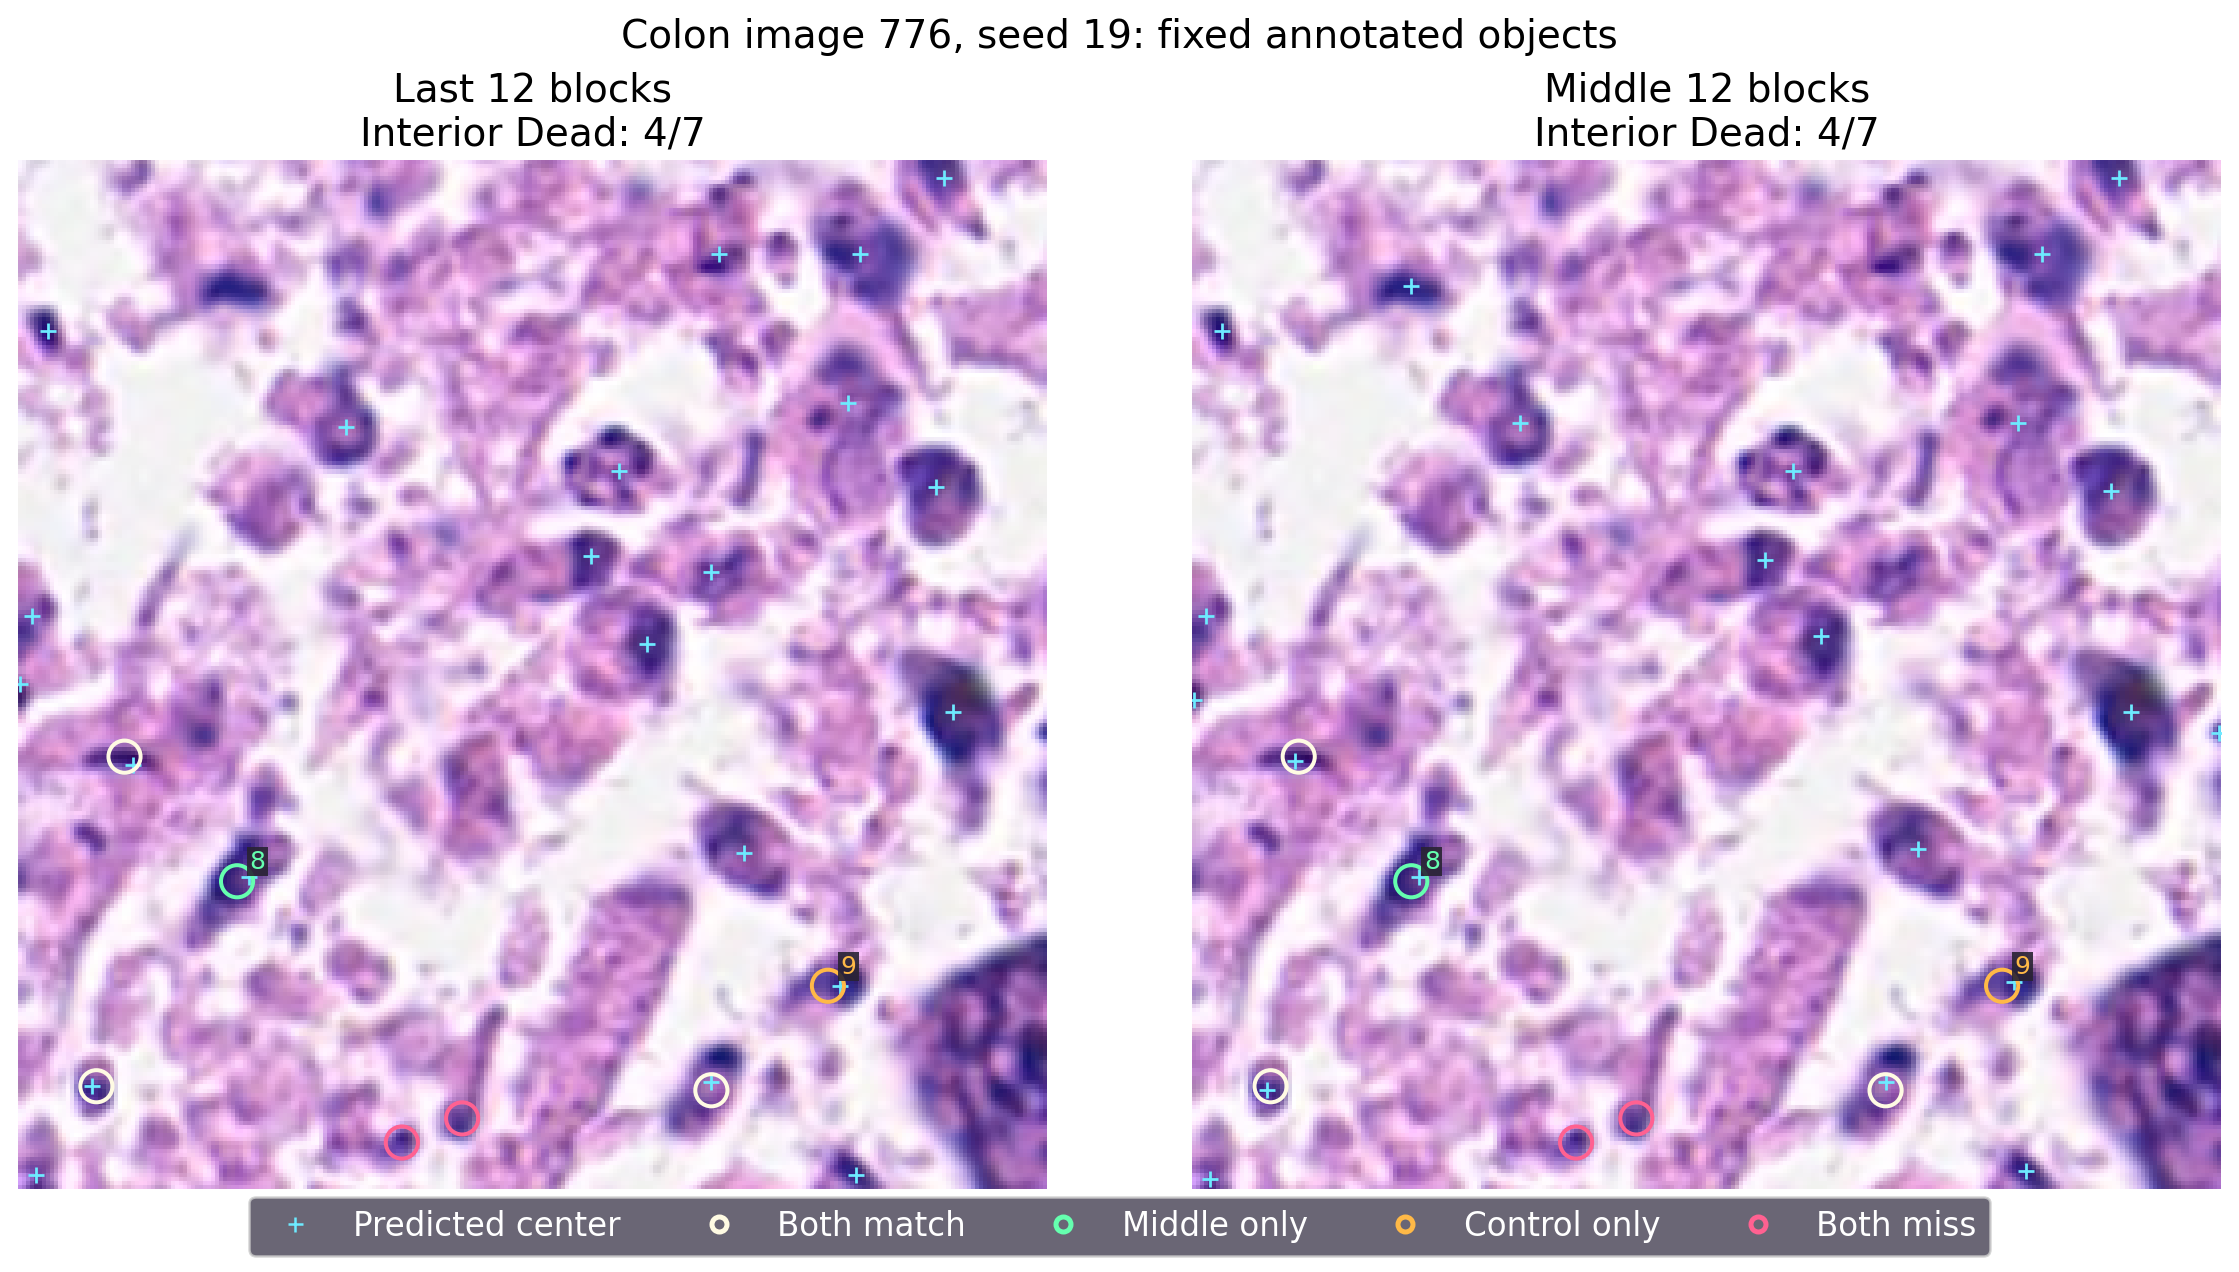
\includegraphics[width=\linewidth,height=.40\textheight,keepaspectratio]{assets/p30_image_776_seed_19.png}
\captionof{figure}{P30, colon image 776, seed 19: unchanged count with exchanged objects. Seed 19; last-twelve control left, middle twelve intervention right. Cyan crosses mark predictions; white, green, orange and pink circles mark matched by both, intervention only, control only and missed by both}
\raggedright

Colon 776 remains at 4/7 while object 8 (179,54) gains, 3.16 → 2.24, and object 9 (205,201) loses, 3.00 → 3.16. Both changes lie near the matching boundary. Seed 1 gains object 9 and improves to 5/7. The unchanged seed-19 count therefore conceals an exchange between annotations. The preserved coordinates measure decoded-point presence and position; probability maps and intermediate feature statistics would allow a direct test of score strength or peak selection in future mechanism work.

\end{minipage}

\subsection{P31: group normalization in the center
detector}\label{p31-group-normalization-in-the-center-detector}

P31 adds eight group-normalization modules to the center detector. For
each image, group normalization calculates feature statistics within
groups of channels and applies learned scaling and offsets. The control
retains the original detector; both models update the last twelve
encoder blocks. The added modules have 2,816 parameters. Data, training
schedule and point matching remain shared with the paired control. All
four runs completed 130 epochs and the results below use the last
checkpoint.

{\def\LTcaptype{none} % do not increment counter
\begin{longtable}[]{@{}
  >{\raggedright\arraybackslash}p{(\linewidth - 10\tabcolsep) * \real{0.1304}}
  >{\raggedleft\arraybackslash}p{(\linewidth - 10\tabcolsep) * \real{0.1739}}
  >{\raggedleft\arraybackslash}p{(\linewidth - 10\tabcolsep) * \real{0.1739}}
  >{\raggedleft\arraybackslash}p{(\linewidth - 10\tabcolsep) * \real{0.1739}}
  >{\raggedleft\arraybackslash}p{(\linewidth - 10\tabcolsep) * \real{0.1739}}
  >{\raggedleft\arraybackslash}p{(\linewidth - 10\tabcolsep) * \real{0.1739}}@{}}
\toprule\noalign{}
\begin{minipage}[b]{\linewidth}\raggedright
Seed and model
\end{minipage} & \begin{minipage}[b]{\linewidth}\raggedleft
Interior Dead matched
\end{minipage} & \begin{minipage}[b]{\linewidth}\raggedleft
Small Dead matched
\end{minipage} & \begin{minipage}[b]{\linewidth}\raggedleft
All matched
\end{minipage} & \begin{minipage}[b]{\linewidth}\raggedleft
Predictions
\end{minipage} & \begin{minipage}[b]{\linewidth}\raggedleft
Precision
\end{minipage} \\
\midrule\noalign{}
\endhead
\bottomrule\noalign{}
\endlastfoot
19, control & 65/145 & 7/32 & 7,274 & 10,536 & 69.04\% \\
19, group normalization & 73/145 & 6/32 & 7,134 & 10,089 & 70.71\% \\
1, control & 68/145 & 9/32 & 7,256 & 10,437 & 69.52\% \\
1, group normalization & 70/145 & 9/32 & 7,262 & 10,354 & 70.14\% \\
\end{longtable}
}

The intervention added 8 and 2 interior Dead matches, changed all
matches by −140 and +6, and reduced unmatched predictions by 307 and 89.
Training-set recall increased from 97.59\%/97.81\% to 99.56\%/99.73\%.
Development Dead recall increased by 5.52/1.38 percentage points; the
paired, tissue-stratified image-bootstrap 95\% intervals were
{[}+3.49,+9.38{]} and {[}−4.30,+4.32{]} points. The original combined
two-seed criterion was not met by either seed.

\noindent

\begin{minipage}{\linewidth}\centering
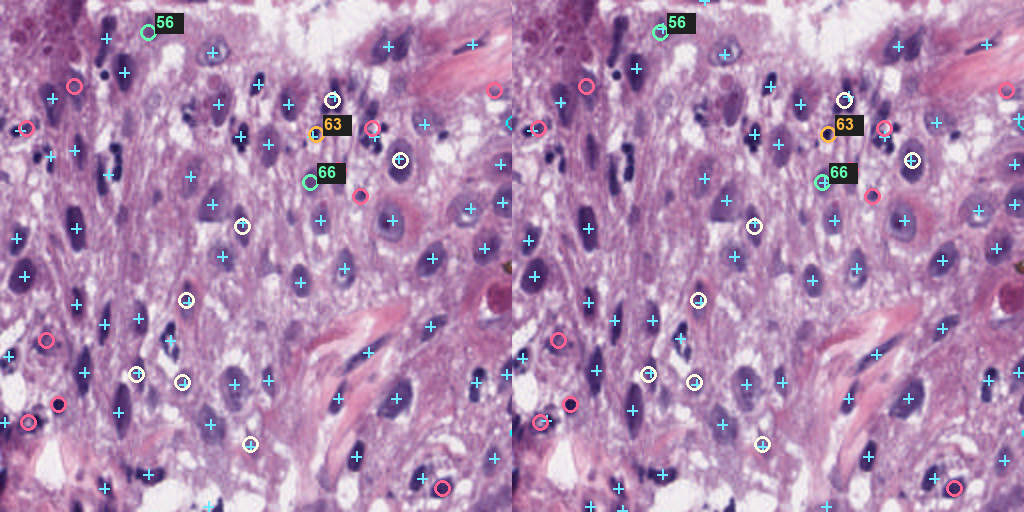
\includegraphics[width=\linewidth,height=.40\textheight,keepaspectratio]{assets/p31_image_1037_seed_19.png}
\captionof{figure}{P31 lung image 1037, seed 19: control left, group normalization right. Cyan crosses are predicted centers; white, green, orange and pink circles indicate matched by both, intervention only, control only and missed by both. Numbers identify annotated objects.}
\raggedright

The image increased from 8/20 to 9/20. Object 56 at row 16, column 74 changed its nearest prediction distance from 21.21 to 2.24 pixels; object 66 at (91,155) changed from 19.65 to 1.00. Object 63 at (67,158) changed from 2.24 to 20.52 pixels and lost its match. The saved coordinates show the appearance and disappearance of nearby predictions.

\end{minipage}

\noindent

\begin{minipage}{\linewidth}\centering
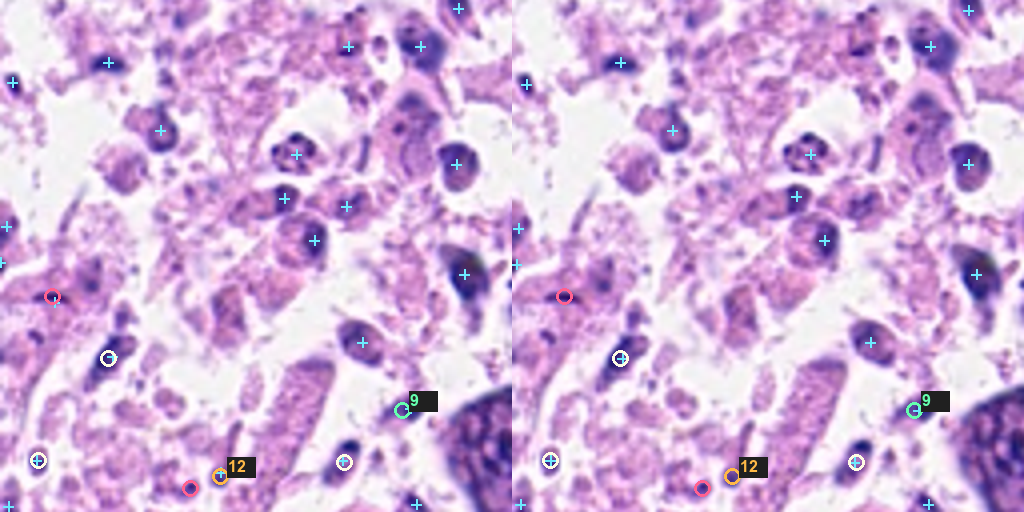
\includegraphics[width=\linewidth,height=.40\textheight,keepaspectratio]{assets/p31_image_776_seed_19.png}
\captionof{figure}{P31 colon image 776, seed 19; control left and group normalization right; cyan crosses are predictions, and white, green, orange and pink circles mark both matched, intervention only, control only and both missed.}
\raggedright

Both models matched 4/7 targets, but exchanged objects. Object 9 at (205,201) moved from 4.12 to 2.00 pixels from the closest prediction; object 12 at (238,110) changed from 2.00 to 61.40 pixels. Both objects were gained in seed 1, where the image rose from 4/7 to 6/7.

\end{minipage}

\noindent

\begin{minipage}{\linewidth}\centering
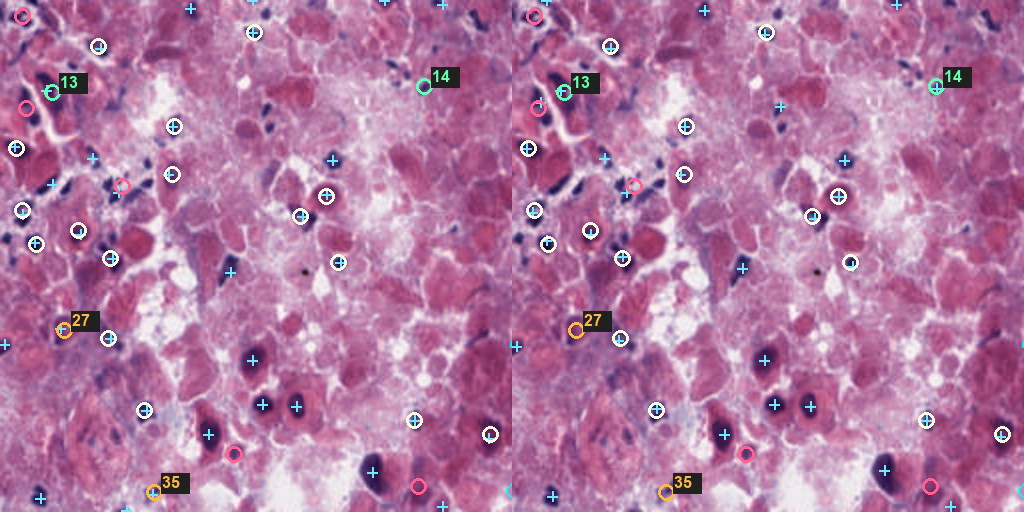
\includegraphics[width=\linewidth,height=.40\textheight,keepaspectratio]{assets/p31_image_1025_seed_1.png}
\captionof{figure}{P31 lung image 1025, seed 1; control left and group normalization right; cyan crosses are predictions, and white, green, orange and pink circles mark both matched, intervention only, control only and both missed.}
\raggedright

The image remained at 18/25. Object 14, with area 31 pixels, gained a prediction at distance 1.00 instead of 41.98; object 13 moved from 3.16 to 2.24. Objects 27 and 35 lost their matches as nearest distances increased from 2.24 and 1.41 to 21.59 and 41.01. The saved images and coordinates describe these changes; measuring their internal causes requires additional model observations.

\end{minipage}

\subsection{Synthesis and evidence}\label{synthesis-and-evidence}

All five rounds use the same development images and a freshly trained
same-seed control in each round. Changing encoder update positions
produces both gained and lost matches within the same image; the
detector change in P31 also exchanges specific objects. Both P29 seeds
added at least 13 interior Dead matches, and both P30 seeds added at
least 516 matches overall. P31 increased detection on training images,
with different development changes between seeds.

The tissue images show fixed examples from the actual outputs. Cyan
crosses are predicted centers; white, green, orange and pink circles
denote annotated Dead nuclei matched by both models, by the intervention
only, by the control only, and by neither. Numbers identify annotations.
Image IDs and coordinates are retained in the evidence directory. All
four P31 runs finished; 92 small files were checked against preservation
manifests, and the subset used here is included. See NUMBER\_SOURCES.md
and README.md for provenance and reproducibility.

\end{document}
